\documentclass[11pt,a4paper,titlepage,spanish]{article}
\usepackage[left=1.5cm,top=2.5cm,right=1.5cm,bottom=2.5cm]{geometry} 
\usepackage[utf8]{inputenc}
\usepackage[spanish, es-tabla]{babel} %esto es para que aparezca "tabla" en lugar de "cuadro" al poner título a una tabla
\usepackage[T1]{fontenc}
\usepackage{booktabs}
%\usepackage{bbm}
\usepackage{amsthm,amsmath,mathrsfs}
\usepackage[hidelinks]{hyperref}
\usepackage[usenames]{color}
\usepackage{subfig}
\usepackage{float}


\usepackage{multirow} % paquete que sirve para la generación de tablas, en especial permite ingresar múltiples filas
\usepackage[table, xcdraw]{xcolor} %para que las celdas de las tablas puedan ser de colores
\usepackage{booktabs} %permite ingresar un formato especial de tablas, es bastante prolijo
\usepackage[stable]{footmisc} %permite poner footnote en los títulos de las secciones

\usepackage[pdftex]{graphicx}
\usepackage{epstopdf}
\DeclareGraphicsExtensions{.pdf,.png,.jpg,.bmp}
\usepackage{pdfpages}

\newcommand{\HRule}{\rule{\linewidth}{0.5mm}}



% --- Para el encabezado
%\usepackage{fancyhdr}
%\fancyhead[L]{Preguntas teoricas} \fancyfoot[C]{\thepage}
%\pagestyle{fancy}
% -------------------------------------------------------- %
%opening
\title{Proyecto de grado\\ ``Análisis de video en Biomecánica''}
\author{Andréi Guchin, Gonzalo Pereira, Guillermo Ottado, Mauricio Ramos. \\
Tutor: Juan Cardelino}
\date {}

\begin{document}

\maketitle

\newpage
\tableofcontents
%\printindex
\newpage

\begin{abstract}
\begin{center}
\begin{minipage}{.8\textwidth}
\chapter*{Resumen}
\addcontentsline{toc} {chapter} {Resumen}%

El objetivo de este proyecto es desarrollar un sistema óptico de captura de movimiento basado en marcadores para facilitar la tarea en el análisis biomecánico del movimiento de las personas.

\vspace{3 mm}

 La propuesta inicial fue realizada por investigadores de biomecánica del Departamento de Biofísica de la Facultad de Medicina de la Universidad de la República, Uruguay, en busca de una herramienta de código abierto que le permita obtener datos y estadísticas específicas que las herramientas existentes no pueden ofrecer.

\vspace{3 mm}

Se elabora una aplicación con los bloques fundamentales que componen un sistema de estas características, utilizando los lenguajes \emph{C/C++}, \emph{Python} y \emph{Matlab}. Estos bloques son independientes unos de otros, lo que da la posibilidad de modificarlos o sustituirlos sin afectar el resto del sistema.

\vspace{3 mm}

También se crea un prototipo de base de datos, con secuencias de videos sintéticas, y un conjunto de algoritmos para medir la performance de cada bloque y del sistema en su totalidad.

\vspace{3 mm}

Las pruebas realizadas sobre el software implementado reflejaron que el mismo tiene una precisión del orden del centímetro. Estos resultados son buenos para ser una primera versión y teniendo en cuenta que los algoritmos utilizados en cada bloque son de complejidad baja y se pueden optimizar en todos sus aspectos.

\end{minipage}
\end{center}
\end{abstract}

\newpage\null\thispagestyle{empty}\newpage

\clearpage
\vspace*{\fill}
\begin{center}
\begin{minipage}{.8\textwidth}
% use section* for acknowledgement
\section*{Agradecimientos}

The authors would like to thank...
\end{minipage}
\end{center}
\vfill % equivalent to \vspace{\fill}

\newpage\null\thispagestyle{empty}\newpage


%%%%%%%%%%%%%%%%%%%%%%%%%%%%%%%%%%%%%%%%%%%%%%%%%%%%%%%%%%%%%%%%%%%%%%%%%%%%%%
%%%%%%%%%%%%%%%%%%%%%%%%%%%%%%%%%%%%%%%%%%%%%%%%%%%%%%%%%%%%%%%%%%%%%%%%%%%%%%
\clearpage
\section{Introducción}
% The very first letter is a 2 line initial drop letter followed
% by the rest of the first word in caps.
% 
% form to use if the first word consists of a single letter:
% \IEEEPARstart{A}{demo} file is ....
% 
% form to use if you need the single drop letter followed by
% normal text (unknown if ever used by IEEE):
% \IEEEPARstart{A}{}demo file is ....
% 
% Some journals put the first two words in caps:
% \IEEEPARstart{T}{his demo} file is ....
% 
% Here we have the typical use of a "T" for an initial drop letter
% and "HIS" in caps to complete the first word.
\IEEEPARstart{T}{his} demo file is intended to serve as a ``starter file''
for IEEE journal papers produced under \LaTeX\ using
IEEEtran.cls version 1.7 and later.
% You must have at least 2 lines in the paragraph with the drop letter
% (should never be an issue)
I wish you the best of success.

\hfill mds
 
\hfill January 11, 2007
\clearpage
\section{Revisión bibliográfica}
\label{invBiblio}

Como se menciona en la introducción, la primer etapa realizada en el proyecto fue la revisión bibliográfica de sistemas de captura de movimiento. Esta primera etapa permite obtener una idea de los distintos procesos que conforman un sistema de captura de movimiento. Estos son:

\begin{itemize}
	\item Calibración.
	\item Adquisición.
	\item Detección de marcadores (Segmentación).
	\item Seguimiento.
	\item Estimación de pose (Reconstrucción).
\end{itemize}

Al no encontrar detalles sobre el diseño de sistemas que verifiquen las hipótesis de este proyecto, o que puedan reutilizarse como base, se decide implementar uno de manera integra, realizando una búsqueda bibliográfica detallada y asignando cada artículo a una categoría de acuerdo a los procesos definidos anteriormente. Esta etapa del proyecto, por momentos tomó carácter de investigación científica más que de proyecto ingenieril. 
En el apéndice I (capítulo \ref{tablabiblio}), se muestra una tabla con toda la bibliografía relevante, ordenada según las categorías antes mencionadas.


En total se clasificaron 18 documentos, dentro de los cuales se encuentran artículos, papers, y publicaciones en general. Los más destacados dentro de cada grupo son:

\begin{itemize}
	\item Calibración.
	\begin{itemize}
		\item \emph{Optical Motion Capture System with Pan-Tilt Camera Tracking and Realtime Data Processing}.
	\end{itemize}
	\item Detección de marcadores (Segmentación).
	\begin{itemize}
		\item \emph{Simple and robust hard cut detection using interframe differences}. En esta investigación se propone un posible algoritmo de segmentación para utilizar en la etapa de detección de marcadores, utilizando un método de detección de bordes. Por motivos que se verán más adelante, estos tipos de algoritmos se descataron para utilizar en segmentación (\textit{ver sección \ref{deteccionMarcadoresSec}}).
		\item \emph{Threshold survey}\cite{surveyThreshold}. Se listan 40 algoritmos de segmentación mediante métodos de umbral. Se evalúan los mismos y se muestran ventajas y desventajas de cada uno. Entre ellos se encuentra el método de umbral de Otsu\cite{otsu}, el cual fue el elegido para implementar en este sistema (\textit{ver sección \ref{deteccionMarcadoresSec}}).
	\end{itemize}
	\item Seguimiento.
	\begin{itemize}
		\item \emph{Skeleton-Based Motion Capture for Robust Reconstruction of Human Motion}\cite{herda}.
		\item \emph{Simple and robust hard cut detection using interframe differences}.
		\item \emph{Modelling and Tracking Articulated Motion from Multiple Camera Views}.
		\item \emph{Skeletal Parameter Estimation from Optical Motion Capture Data}.
		\item \emph{Optical Motion Capture System with Pan-Tilt Camera Tracking and  Realtime Data Processing}.
		\item \emph{Resolving Motion Correspondence for Densely Moving Points}.
	\end{itemize}
	\item Estimación de pose (Reconstrucción).
	\begin{itemize}
		\item \emph{Skeleton-Based Motion Capture for Robust Reconstruction of Human Motion}\cite{herda}.
		\item \emph{Modelling and Tracking Articulated Motion from Multiple Camera Views}.
		\item \emph{Skeletal Parameter Estimation from Optical Motion Capture Data}.
		\item \emph{Optical Motion Capture System with Pan-Tilt Camera Tracking and  Realtime Data Processing}.
		\item \emph{What can two images tell us about a third one?}.
	\end{itemize}
	\item Sistemas completos
	\begin{itemize}
		\item \emph{Detección, rastreo y reconstrucción tridimensional de marcadores pasivos para análisis de movimiento humano}.
		\item \emph{Marker Detection and trayectory generation algorithms for a multicamera based gait analysis system}.
		\item \emph{Analisis de video para estimacion del movimiento humano}.
	\end{itemize}
\end{itemize}

Se puede ver, que en varios casos un mismo artículo contiene información de valor sobre varias etapas del sistema. Además se encontraron algunos documentos con diseños de sistemas completos.

A partir de esta etapa se definieron ciertos aspectos de vital importancia para el proyecto, en particular, se pudo seleccionar para el bloque de detección de marcadores el método de segmentación por umbral dinámico de Otsu\cite{otsu}. Este método fue elegido por tener el mejor compromiso entre simplicidad y eficacia.

En los bloques de seguimiento y estimación de pose se decide basar el desarrollo en las ideas del sistema propuesto por Lorna Herda en sus tesis de doctorado\cite{herda}. Dicha elección se debe a que el estudio de Herda contiene las ideas principales para implementar un sistema de captura de movimiento de manera compacta y general, posee una gran cantidad de menciones siendo un referente en el tema y la documentación disponible es amplia (dos papers, y tesis completa). Por otro lado, dicho trabajo se encuentra bajo las mismas hipótesis de uso que el estudio preliminar realizado por este equipo de proyecto (uso en fisioterapia, animación, biomecánica, entrenamiento en alto rendimiento), y es un punto de referencia habitualmente mencionado. Sin embargo, si bien en todas sus menciones la metodología de tratamiento de datos es la misma, tanto los bloques de adquisición como de detección van variando en equipamiento y métodos en los distintos proyectos.
\clearpage
\section{Base de datos} \label{section_base_de_datos}


\subsection{Introducción} SECCION EN CONSTRUCCION\\
MENCIONAR QUE TIPO DE BASE DE DATOS SE NECESITA ENCONTRAR\\
Con el fin de relevar distinta clases de actividades humanas y en particular la marcha, se pretende trabajar con una base de datos basada en marcadores, que contenga un cierto número de sujetos, realizando una variedad de movimientos predefinidos, donde para cada sujeto a estudiar, se tengan múltiples secuencias de videos 2D del movimiento obtenidas a partir de cámaras situadas en un entorno 3D cerrado previamente acondicionado. Dicha base debe contar con el correspondiente ground truth 2D y 3D de los datos de movimiento relevados, en nuestro caso como nuestro sistema está basado en marcadores, dicha información consiste en obtener las coordenadas espaciales a lo largo del tiempo para cada marcador de interés. Así como la información de calibración.blablabla MEJORAR \\

MENCIONAR PORQUE SE TUVO QUE GENERAR UNA Y QUE CONTIENE A GRANDES RASGOS\\
Se propone una estructura de datos para almacenar la información relevante del ground truth y  se cuenta con código de soporte que facilita la generación de nuevas secuencias así como la gestión de la información en la estructura de datos, evaluar resultados y realizar el  posterior análisis de performance.


blablablabl
Un ambiente controlado con cámaras ajustadas convenientemente provee un escenario ideal para obtener información óptica de los marcadores. El sujeto es condicionado a moverse sobre un espacio de captura determinado con una vestimenta particular; la elección adecuada de estos parámetros junto con las condiciones de iluminación y el tipo de fondo facilitan la recolección de información, el posterior análisis y sobre todo aumentan la performance del sistema completo.
\\COMBINAR LO ANTERIOR CON ESTO
Necesitamos una base de datos para implementar, testear y comparar los distintos tipos de algoritmos desarrollados. Por lo tanto es de interés primario relevar las bases de datos existentes o en su defecto realizar una.\\
Para ello en primera instancia se buscaron bases de datos en la web. La búsqueda se centro en encontrar secuencias de video de personas caminando donde, dada las características de nuestro proyecto, las mismas deben poseer marcadores claramente distinguibles. Las secuencias deben ser tomadas con varias cámaras ubicadas alrededor del sujeto y para obtener información 3D como mínimo la cantidad de cámaras deben ser dos. Además se debe tener el ground truth con la posición espacial de dichos marcadores para testear y comparar los distintos algoritmos de seguimiento aplicados sobre dichas secuencias


\subsection{Revisión de base de datos}
\label{}
En esta sección se muestra  resultados del relevamiento de bases de datos útiles para el análisis de la marcha.
Inicialmente nuestro objetivo era obtener un sistema funcional para el caso de la marcha humana, aunque luego de la implementación del mismo se generalizaron sus usos, las bases de datos con este tipo de movimiento fueron el eje central de la búsqueda.

Se encontraron principalmente tres páginas web que a manera de compendio agrupan  bases de datos útiles en varias de las ramas de la visión por computadora.\\

\hspace{-0.7cm} \textbf{CVonline \footnote{\textcolor{blue}{\underline{\url{http://homepages.inf.ed.ac.uk/rbf/CVonline}}}. Accedido 30-11-14.} } 

Bastante completa, no solo contiene enlaces a  varias bases de datos sino reune bibliografía e implementaciones útiles.\\


\hspace{-0.7cm} \textbf{Computer Vision Papers \footnote{\textcolor{blue}{\underline{\url{ http://www.cvpapers.com/datasets.html}}}. Accedido 30-11-14.} } 

	 Solo reúne enlaces de bases de datos.\\
		

\hspace{-0.7cm} \textbf{Yet Another Computer Vision Index To Datasets (YACVID)} \footnote{\textcolor{blue}{\underline{\url{http://riemenschneider.hayko.at/vision/dataset/}}}. Accedido 30-11-14. } 	

Una característica importante es que la página contiene direcciones a bases de datos relativamente nuevas y resalta aquellas que son usadas con mayor frecuencia. \\
	

Dentro de estas páginas se encuentra una gran variedad de bases de datos que tratan el caso particular de la marcha, en la tabla \ref{bases_relevadas} se muestran algunas de las bases relevadas y sus características representativas, que permiten hacer una idea del panorama global encontrado a la hora de recopilar información en la web.  

\begin{table}[h!]
	\centering	
	\caption{Comparación de algunas bases de datos disponibles y empleadas por la comunidad.}
	\label{bases_relevadas}
	\begin{minipage}{\textwidth} %por algún motivo el arabic no funciona, no me pone llamados a pie de página numericos	
	\begin{tabular}{||l|ccccc||} 
\hline
\rowcolor[HTML]{CBCEFB} 

\textbf{Base}     & \textbf{Cantidad }  & \textbf{Nro. de }   & \textbf{Entorno} & \textbf{Número de} & \textbf{Calibración}\\
\rowcolor[HTML]{CBCEFB} 
\textbf{de datos} & \textbf{de sujetos} & \textbf{secuencias} &         & \textbf{cámaras }  &  \textbf{disponible} \\


\hline \hline
M.C.L.\footnote{Motion Capture Lab}  & 3 		& 		299	   & Interior&     1    &    No      \\ \hline
C.M.U  \footnote{Carnegie Mellon University Motion Capture Database}	
 & >100     &       2605   & Interior&      1   &    No       \\ \hline
G.T \footnote{Georgia Tech} &       20    & $\sim$100           & Interior y &   3      &  Si       \\ 
	 &		 &					 & exterior        &         &    \\ \hline
U.S. \footnote{University of Southampton Database} &       >100    &     $\sim$ \footnote{El símbolo $\sim$ indica que no se cuenta con información al respecto.}  & Interior &   12      &  $\sim$      \\ \hline
Human ID  &     122    & 1870           & Exterior &   2      &$\sim$       \\ \hline
HumanEva &     4+2    & 56           & Interior &   4/7      &  Si       \\ \hline
INRIA \footnote{INRIA Perception, Multicam Dataset. } &       >11    & >40           & Interior &   $\geq$1      &  Si       \\ \hline
CMU Mobo \footnote{CMU Motion of Body.} &     25    & 100           & Caminadora &   6      &  $\sim$       \\ \hline
CASIA &     385    & $\sim$           & Interior y  &   >4      &  $\sim$       \\ 
&         &            & exterior  &         &      \\ \hline
MHAD \footnote{Berkeley Multimodal Human Action Database.} & 12         & 660            & interior  & 12        & Si      \\ 
\hline \hline


\rowcolor[HTML]{CBCEFB}
\textbf{Base}     & \textbf{Movimientos}  & \textbf{Apariencia}    & \textbf{Ground Truth} & \textbf{Tipo}  & \\
\rowcolor[HTML]{CBCEFB}
\textbf{de datos} & \textbf{disponibles} &               &           & \textbf{de acceso} & \\
\hline \hline
{M.C.L. }   & Varios    &  Traje MoCap & 3D-Vicon \footnote{ Esta notación indica que la captura considerada ground truth, se hizo con un sistema  de captura de movimiento (MoCap) de Vicon-Peak, \textcolor{blue}{\underline{\url{http://www.vicon.com/}}} } & Libre & \\ \hline
{C.M.U }    & Varios    &  Traje MoCap & 3D-Vicon \footnote{Secuencias bvh de CMU, \textcolor{blue}{\underline{\url{http://sites.google.com/a/cgspeed.com/cgspeed/motion-capture}}}.} & & \\ \hline
{G.T} &     Marcha fuera&     Traje MoCap y       & 3D  en formato & Libre & \\ 
 &	   de régimen  &  Natural   &   Maya & & \\ \hline
U.S. &       Marcha    &  Natural    &  $\sim$ Libre&       \\	\hline
Human ID &     Marcha    & Natural  & $\sim$ & Bajo  &       \\ 
						 &        &   &  & solicitud &       \\ \hline
HumanEva &     Varios    & Natural  & 3D - Vicon & Bajo  &       \\ 
						 &        &   &  & solicitud &       \\ \hline
INRIA &       Varios    & Traje MoCap y            & 2D - MoCap &  Libre &       \\
&           & Natural            &   etiquetado manual  & &         \\ \hline
CMU Mobo &     5 tipos de marcha    & $\sim$           & Etiquetado Manual \footnote{Disponible en  \textcolor{blue}{\underline{\url{http://www.cs.cmu.edu/~zhangjy/\# Data}}}.}& Bajo  &       \\ 
 							 &        &   &  & solicitud &       \\ \hline
CASIA &  Varias velocidades       &   Natural         & No  &    Bajo     &      \\ 
& de marcha        &            &   & solicitud        &      \\ \hline
MHAD & Varios        & Traje MoCap            & 3D - Impulse \footnote{ Esta notación indica que la captura considerada ground truth, se hizo con un sistema  de captura de movimiento (MoCap) Impulse (PhaseSpace Inc., San Leandro, CA), \textcolor{blue}{\underline{\url{http://www.phasespace.com/}}} }    & Libre  &       \\
\hline
	\end{tabular}
	\end{minipage}	
\end{table}

A continuación algunos comentarios que vale la pena resaltar sobre  las bases anteriores.

\paragraph{Motion Capture Lab.\footnote{\textcolor{blue}{\underline{\url{http://accad.osu.edu/research/mocap/mocap_home.htm}}}. Accedido 30-11-14}} 
		Como describe el nombre, este laboratorio se centra en obtener capturas de movimiento tridimensionales a través del sistema Vicon. Cuentan con un sistema Vicon 8i de 14 cámaras, dos videocámaras digitales Sony DSR-PD150 que llegan a 30 fps\footnote{\textcolor{blue}{\underline{\url{http://www.bhphotovideo.com/c/product/197878-REG/Sony_DSRPD150_DSR_PD150_Professional_1_3_DVCAM.html}}} ,Accedido 29-11-14 }, junto a un sistema de sincronización que permite integrar todas estas cámaras en el laboratorio. El video se utiliza únicamente como ayuda en los datos de captura para corregir y ver los marcadores,  por lo que \underline{no cuenta con secuencias de video adecuadas}. Cabe destacar que maneja múltiples formatos MoCap, inclusive el bvh.

\paragraph{Carnegie Mellon University Motion Capture Database.\footnote{\textcolor{blue}{\underline{\url{http://mocap.cs.cmu.edu/}}}. Accedido 30-11-14}}\label{CMU}
 Este laboratorio también se centra en obtener capturas de movimiento a través de un sistema Vicon, y no está implementado para evaluaciones ópticas de las capturas. Solo maneja videos monoculares de baja resolución, por lo que no cuenta con secuencias de video adecuadas para nuestro proyecto. Sin embargo maneja múltiples formatos MoCap y  posee herramientas para conversión a otros formatos, incluido el bvh. Posee descripción detallada de la ubicación de los marcadores, así como de la configuración del laboratorio. El sujeto a relevar se encuentra vestido con ropas finas y ajustadas, sobre la cual se colocan los marcadores, por lo tanto se puede despreciar las fluctuaciones de posición de marcadores debidas a la ropa, que si exhiben otros ambientes menos controlados  Esta base de datos es bastante utilizada en el ámbito de la  animación por computadora y es por lejos la que dispone de mayor cantidad de capturas de movimiento de acceso público de las bases relevadas en esta sección.

\paragraph{Georgia Tech.\footnote{\textcolor{blue}{\underline{\url{http://www.cc.gatech.edu/cpl/projects/hid/index.html}}}. Accedido 30-11-14}}
Se encuentra desarrollando maneras de identificar a los seres humanos a distancia a través del reconocimiento de la marcha. También llevan a cabo trabajos relacionados en la localización y seguimiento de rostros, la detección de oclusiones y actividades específicas de sustracción de fondo.
Lamentablemente las cámaras están todas sobre un costado del caminante, la resolución es baja y no todos los videos poseen marcadores. No se cuidan las condiciones de laboratorio para trabajar de manera óptica según nuestras necesidades.


\paragraph{University of Southampton Database.\footnote{ \textcolor{blue}{\underline{\url{http://www.gait.ecs.soton.ac.uk/database}}}. Accedido 30-11-14}}\label{U.S.}
Interesados en el reconocimiento de personas a través del seguimiento de la marcha, relevantes sobre todo por ser pioneros en el estudio biomecánico de la marcha. Poseen dos bases de datos, HiD gait database  (100 sujetos) y Biometric tunnel. El servidor donde se alojaba la base de datos está fuera de línea desde el 2004, el encargado de la página es Mark Nixon (\textcolor{blue}{\underline{\url{msn@ecs.soton.ac.uk}}}). Aparentemente se continúa actualmente el proyecto en \textcolor{blue}{\underline{\url{http://www.cspc.ecs.soton.ac.uk/gait}}}\footnote{Accedido 30-11-14}. Si bien estas bases de datos no están basadas en marcadores, cabe resaltar que el fondo del espacio de captura del túnel biométrico contiene patrones asimétricos con colores saturados que facilitan no solo la extracción de fondo sino también la automatización del proceso de calibración.

\paragraph{Human ID Gait Challenge Dataset.\footnote{\textcolor{blue}{\underline{\url{http://marathon.csee.usf.edu/GaitBaseline/ }}}. Accedido 30-11-14} }
Contiene 1.2 Tera bytes de información. Utilizada para el reconocimiento de la marcha,  no posee marcadores. Al igual que en la base de Southampton contiene en la secuencia imágenes de dameros convenientemente dispuestos, útiles para calibrar las cámaras. Las sucesivas secuencias tomadas para un mismo sujeto modifican distintos tipos de factores, como la calidad del terreno a recorrer, si el sujeto lleva o no un maletín y el  tipo de calzado utilizado. Tienen disponible junto a todas las secuencias de la base de datos las siluetas de los sujetos, obtenidas con un algoritmo base también propuesto y disponible. Lamentablemente el enlace que indica el protocolo seguido para obtener secuencias, junto con la especificación del equipamiento, está fuera de línea.

\paragraph{HumanEva.\footnote{\textcolor{blue}{\underline{\url{http://vision.cs.brown.edu/humaneva/index.html }}}. Accedido 30-11-14} \cite{humaneva} }
Con 1.6 Gigabytes de información, el trabajo de este laboratorio es muy completo, incluye métricas de evaluación y un análisis importante de las necesidades actuales a la hora de generar una base de datos para relevar actividades humanas. El único inconveniente para cumplir los requisitos de nuestro proyecto es que no está pensado para el seguimiento óptico de marcadores, por lo que los marcadores sobre los sujetos de estudio utilizados para recabar datos Mocap son escasos y demasiado pequeños, las condiciones de luminosidad y color de fondo no son las adecuadas para nuestro propósito, incluso utilizan máscaras sobre las imágenes ópticas para cubrir los marcadores, estos últimos son utilizados solo para recopilar el ground truth a través de un sistema Vicon.  Dado que su motivación es obtener una imagen ``natural'' del sujeto que contenga la complejidad generada por el movimiento de la ropa, el ground truth que presentan  no es tan preciso como los obtenidos por métodos más tradicionales.  Contiene código para efectuar sustracción de fondo y la implementación de un algoritmo base, con un filtrado de partículas utilizado para el seguimiento de la pose del sujeto. Para acceder a los datos se debe gestionar un permiso en la página de HumanEva. 

\paragraph{INRIA Perception, Multicam Dataset.\footnote{INRIA Perception, Multicam Dataset, \textcolor{blue}{\underline{\url{http://4drepository.inrialpes.fr/pages/home}}}. Accedido 30-11-14}} Efectúan las capturas con múltiples cámaras y también ofrecen la secuencia de malla de los sujetos reconstruidos a partir de las imágenes. Ofrecen un software que permite navegar en 4D, es decir, el espacio y el tiempo, sobre los modelos disponibles en su base de datos. Por lo que estos modelos se pueden ver desde cualquier ángulo de visión e inspeccionar congelándolos en cualquier instante de tiempo. Lamentablemente su captura no está basada en marcadores. 

\paragraph{CMU MoBo Dataset.\footnote{CMU Motion of Body,  \textcolor{blue}{\underline{\url{http://www.ri.cmu.edu/publication_view.html?pub_id=3904}}}. Accedido 30-11-14}}
Estudia la marcha humana, enfocada en la identificación Biométrica de humanos a partir de sus características individuales. Los sujetos bajo estudio efectúan 4 tipos de caminata sobre una caminadora: marcha lenta, marcha rápida, marcha sobre plano inclinado y marcha sosteniendo un balón. Se utilizan 6 cámaras de alta resolución ubicadas alrededor de la caminadora que adquieren imagenes a 30 frames/s. Para acceder a la base de datos debe pedirse acceso comunicandose con \textcolor{blue}{\underline{\url{rgross@cs.cmu.edu }}}

\paragraph{CASIA Gait Database.\footnote{ \textcolor{blue}{\underline{\url{http://www.cbsr.ia.ac.cn/english/Gait\%20Databases.asp
 }}}. Accedido 30-11-14}} 
Contiene 4 bases de datos sobre la marcha, la primera se efectúa en exteriores y posee una sola cámara; la segunda es en interiores  y posee 11 cámaras sobre un lado del sujeto; la tercera utiliza cámaras infrarrojas y cada sujeto efectúa tres tipo de marcha, lenta, rápida y con mochila; por último la cuarta combina la información de cámaras de captura con una plataforma que registra la presión de la planta del pie a medida que el sujeto desarrolla el movimiento. Además de los archivos de vídeo, ofrecen las siluetas humanas a partir de sus secuencias de vídeo. Las capturas visuales no están basadas en marcadores.

\paragraph{Berkeley Multimodal Human Action Database (MHAD).\footnote{\textcolor{blue}{\underline{\url{http://tele-immersion.citris-uc.org/berkeley_mhad\#dl  }}}. Accedido 30-11-14}}
El objetivo de esta base de datos es reconocer el movimiento del cuerpo al realizar este distintas actividades. Tiene la información necesaria para efectuar sustracción de fondo, devuelven información desde múltiples fuentes:
\begin{itemize}
\item sistema con 12 cámaras ópticas agrupadas en 4 conjuntos de cámaras estéreo
\item dos sensores Kinect
\item 6 acelerómetros sobre el sujeto
\item 4 micrófonos a cada lado del espacio de captura
\end{itemize} Todas estas fuentes se encuentran sincronizadas. Esta base de datos es bastante completa en cuanto a los tipos de captura que realiza, pero los marcadores utilizados son leds y únicamente se utilizan para recabar información para el ground truth, con lo cual no se cuida de obtener una buena información óptica de los mismos. 



\subsubsection{Contactos realizados y resultados} 
En el ámbito local hemos estado en contacto con la magister Patricia Polero, quien nos ha brindado su experiencia previa en el tema de capturas ópticas de movimiento basadas en marcadores así como ayudado a definir los requerimientos mínimos del sistema a implementar  en las etapas iniciales. También se han generado reuniones con Darío Santos, Fisioterapeuta en el Hospital de Clínicas, quien actualmente ¿dirije? un laboratorio que posee un sistema de captura de movimiento basado XXXX el cual han adquirido recientemente. Si bien dicho sistema pudo haber sido primordial para generar una base de datos con secuencias reales, no se pudo coordinar debidamente su uso. De todas maneras en estas reuniones, se obtiene un reducido número de secuencias relativamente útiles. Cabe destacar que las mismas no poseen la calidad deseada, por pertenecer a versiones previas del laboratorio cuando aún no disponían del sistema actual, así como tampoco cumplen la totalidad de supuestos sobre las condiciones de captura planteados al inicio del proyecto. 


Los pedidos se realizan a partir del 17 de diciembre de 2013 aproximadamente. En los mismos se intenta gestionar el acceso a las bases de datos de acceso restringido, que entendimos poseen características útiles en el desarrollo de nuestro sistema. En la tabla \ref{tabla_solicitudes} se muestran los contactos realizados y los resultados obtenidos.


\begin{table}[h]
	\centering		
	\begin{tabular}{@{}lr@{}} 
	\toprule		
	\multicolumn{1}{l}{\textbf{Base de datos}} & \textbf{Resultados }\\	
	\midrule
	HumanEva		&	concedida 27 julio 2014\\
	CASIA			&	concedida 3 de mayo 2014\\
	CMU Mobo		&	sin respuesta \\
	\midrule
	\multicolumn{1}{l}{\textbf{Escasas secuencias de video}} & \textbf{Resultados }\\
	\begin{tabular}[l]{@{}l@{}}Darío Santos,\\ Depto. Fisiatría Y
	Rehabilitación.\\ Hospital de Clínicas.\end{tabular}	&	concedida 29 julio 2014\\	
	\bottomrule
	\end{tabular}
	\caption{Solicitudes de acceso gestionadas.}
	\label{tabla_solicitudes}	
\end{table}



\subsubsection{Conclusiones}\label{conclusiones_revision_base_datos} SECCION EN CONSTRUCCION\\

Si bien se encontraron numerosas bases de datos para la marcha, todas ellas terminan siendo descartadas por no ajustarse completamente a las hipótesis bajo las cuales se trabaja en este proyecto. Deficiencias tales como la inadecuada cantidad o posición de las cámaras, condiciones del laboratorio que dificultan y en algunos casos imposibilitan una correcta segmentación a partir de la información óptica. Y por último la ausencia o tamaño inadecuado de los marcadores. Son los factores más importantes.
Salvando diferencias, el problema principal está en que no se tienen imágenes ópticas para trabajar con marcadores, en general se tiende a trabajar sobre el cuerpo completo, y se contrasta el procesamiento con datos Mocap relevados con sistemas infrarrojos. Por otro lado esto último genera una rica fuente de material de trayectorias de puntos 3D en distinto tipo de movimientos, sobre todo en formatos Mocap.
Estas consideraciones impulsaron la idea de recorrer el camino inverso, crear una base de datos sintética a partir del material Mocap disponible, para luego generar los videos en los cuales trabajar.  







Si bien la búsqueda se centró en blablabla no logró encontrar una base de datos que cumpliera las especificaciones de nuestro proyecto. Debido a blablabla SEGUIMIENTO OPTICO DE MARCADORES.
 De todas maneras se genera un relevamiento de bases de datos para el movimiento humano, se profundiza en las características usuales que presentan dichas bases de datos y se logra reunir un conjunto de conceptos y herramientas necesarios para introducirnos en el tema. 

% % % % % % % % % % % % % % % % % % % % % % % % % % % % % % % % % % % % % % % % % % % % % % % % % % % % % % % % % %
% % % % % % % % % % % % % % % % % % % % % % % % % % % % % % % % % % % % % % % % % % % % % % % % % % % % % % % % % % %5


\subsection{Características de Laboratorio para un sistema de captura óptica basado en marcadores}
\label{seccion_Caracteristicas_Laboratorio}
 
A continuación se enumeran algunas variables que es necesario tener en cuenta a la hora de diseñar un Laboratorio, adecuado para un sistema de captura óptica basado en marcadores. También se discute brevemente el posible impacto de estás variables en el tratamiento posterior de las secuencias.

\subsubsection{Cámaras}\label{parrafo_Camaras} 
Para la elección del tipo de cámaras es importante tener en cuenta los requerimientos de las secuencias a relevar. A continuación vamos a tratar dos variables básicas y generales que deben contemplarse, por un lado la cantidad de fotogramas, y por otro la resolución de la cámara.

La cantidad de fotogramas por segundo de las secuencias de video condiciona la resolución temporal de los datos procesados a partir de dichas secuencias, así como también limita la velocidad de movimiento a realizar por el sujeto si se busca una captura aceptable.
Basados en el relevamiento de las distintas bases de datos se puede afirmar que 30fps es un valor normal para trabajar el caso de la marcha, pudiendo obtener en este caso información de la posición de los marcadores solo cada 1/30 segundos.\\ 
Hay que tener presente que si se efectúan movimientos de velocidades superiores a la marcha, manteniendo la cantidad de fotogramas anterior, aumenta la dificultad a la hora de vincular temporalmente los datos obtenidos, pudiendo bajar la performance del seguimiento de los marcadores. 

Respecto a los tiempos de obturación, estos deben ser bastante cortos  para no producir efectos de desplazamiento nocivos a la hora de reconocer los marcadores.
Una regla habitualmente utilizada que sirve de orientación es que el tiempo mínimo de disparo que asegura que no salga movida una imagen, es la inversa de la distancia focal. También se encuentran referencias que indican los tiempos de obturación recomendados según la actividad a relevar. \footnote{\textcolor{blue}{\underline{\url{http://es.wikipedia.org/wiki/Velocidad_de_obturación}}}}.
\begin{itemize}
\item $1 / 4000~ s$:  se utiliza para tomar fotografías nítidas de sujetos en rápido movimiento, como los atletas o vehículos, en condiciones de buena iluminación.
\item $1 / 2000 ~s$ y $1/ 1000~s$: útil  para fotografías nítidas de sujetos en movimiento moderadamente rápido, bajo condiciones normales de iluminación.
\item $1 / 500~s$ y $1/ 250~s$ :  para tomar fotografías nítidas de personas en movimiento en situaciones cotidianas.
\end{itemize}
 
 
 La resolución del sensor también juega un rol fundamental a la hora de cumplir requerimientos de resolución espacial en los datos de salida.
 En la figura \ref{estimacion_resolucion} se hace un bosquejo que permite estimar la resolución espacial a medida que el sujeto se aleja de la cámara.
 
\begin{figure}[H]
  \centering
  {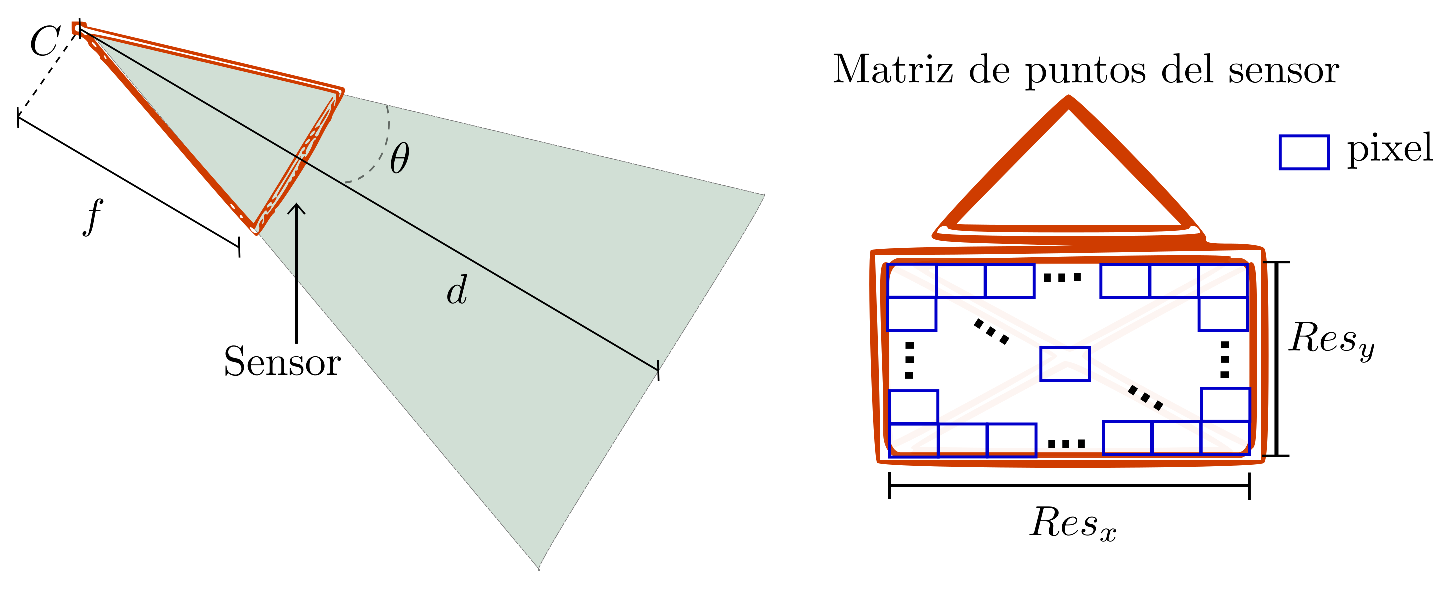
\includegraphics[scale=0.5]{img/Base_Datos/camara_resolucion.eps}}      
  \caption{Estimación del la resolución espacial.}
  \label{estimacion_resolucion}
\end{figure} 

Llamemos $x_s$ e $y_s$ a magnitudes sobre el sensor de la cámara, horizontal y vertical respectivamente, y sea $X$ e $Y$ las magnitudes a una distancia $d$ del centro $C$ de la cámara que producen respectivamente las proyecciones de magnitud $x$ e $y$ sobre el sensor.
Se cumple la siguiente relación,
\begin{alignat*}{1}
X = \dfrac{d}{f}x_s&~, \quad \quad Y = \dfrac{d}{f}y_s
\end{alignat*}

Si el sensor\footnote{También referido como retina de la cámara.} tiene un largo $S_x$ y ancho $S_y$ y resolución de $R_x\times R_y$ píxeles, resulta que el largo de un pixel es $l_x = S_x/R_x $ y el ancho $l_y = S_y/ R_y$. 

A modo de ejemplo consideremos una cámara con las siguientes características $S_x = 0.032\;m$ y $S_y = 0.010\; m$, resolución de $1600\times600$ píxeles y una distancia focal de $32~mm$. Por lo tanto el error de un píxel se mapea sobre el sensor como $x = 0,032/1600\;m = 0.020\;mm$ a lo largo, e $y = 0.010/600\;m= 0.016\;mm$ a lo ancho. La tabla \ref{table_resolucion} muestra como  errores de 1, 2 y 3 píxeles en el sensor se propagan sobre el espacio a una distancia $d$ del centro de la cámara.
\begin{table}[h]
\centering
\begin{tabular}{|c|l|l|l|l|l|}
\hline
\multirow{2}{*}{\begin{tabular}[c]{@{}c@{}}\textbf{número} \\\textbf{ de píxeles}\end{tabular}} & \multicolumn{5}{c|}{\textbf{d (metros)}} \\ \cline{2-6} 
                                                                              &\textbf{ 0,5}  &\textbf{ 1,0}  & \textbf{3,0}  & \textbf{5,0} & \textbf{10,0}\\ \hline
\textbf{1}                                                                             &  0,03    &  0,06    &   0,19   &  0,31   & 0,63      \\ \hline
\textbf{2}                                                                             &  0,06    &  0,12    &  0,38    &  0,62   &  1,26    \\ \hline
\textbf{3}                                                                            &   0,09   &  0,18    &  0,57    & 0,93    &  1.89    \\ \hline
\end{tabular}
\caption{Resolución espacial en centímetros como función de la distancia al centro de la cámara}
\label{table_resolucion}
\end{table}


\subsubsection{Marcadores}
A la hora de seleccionar el equipamiento se debe prestar especial atención y coordinar el tipo de marcador, la vestimenta del sujeto, el fondo del espacio de captura y el tipo de iluminación. Pues las características de estos elementos en conjunto pueden cambiar sensiblemente la performance del sistema que procesa computacionalmente la captura, sobre todo en sus primeras etapas tales como la detección de marcadores y la  calibración.
Si se quiere facilitar la tarea de detección automática de marcadores, estos deben ser fácilmente distinguibles del resto del entorno, y visibles la mayor cantidad de tiempo para las cámaras. Para ello se debe tener marcadores que generen un alto contraste con el resto de los elementos dentro de la captura de video. 
Su tamaño y forma también son importantes, por lo general se trabaja con marcadores esféricos, y un tamaño que dado cierto espacio de trabajo no condicione fuertemente la resolución necesaria de las cámaras. Una medida que se puede considerar aceptable con cámaras convencionales y movimientos a menos de 12 metros del centro de las cámaras, son marcadores de $3~cm$ de diámetro.  
Si el fondo del espacio de captura es negro, opaco, al igual que la vestimenta del sujeto a capturar, los marcadores pueden ser blancos, no pulidos de manera que su reflejo sea difuso, para no generar variación de tono sobre los mismos. 
Su disposición sobre el sujeto responde a los intereses de lo que se quiera observar, pero se debe tener presente que al ser una captura óptica, para que un marcador sea útil, debe estar visibles buena parte del tiempo en la secuencia.

\subsubsection{Iluminación}
La iluminación debería ser preferiblemente uniforme, para no generar sombras que modifiquen los tonos del espacio de captura. La luz natural es una buena alternativa, en espacios cerrados lo que habitualmente se utilizan son pantallas delante de los focos lumínicos para hacerlos más difusos, reduciendo así el riesgo de generar imágenes especulares en los objetos. La disposición de los focos depende de la forma del espacio de captura, pero por lo general rodean al mismo, cuidando que estos no sean capturados directamente por las cámaras, y generen falsos positivos en la detección de marcadores. Si bien esto último puede ser solucionado parcialmente en la etapa de  post-procesamiento efectuando convenientemente sustracción de fondo, es recomendable tratarlo en las primeras etapas, a nivel del sistema de captura. 

\subsubsection{Vestimenta}
Es preferible que la vestimenta del sujeto a relevar, consista en ropas finas y ajustadas para despreciar fluctuaciones de la posición de marcadores debido al movimiento de la ropa. Como se menciona anteriormente al igual que el fondo, la elección del color y material debe contrastar con los marcadores.

\subsubsection{Espacio de captura}

Ya se ha mencionado algunas características cualitativas relacionadas con el espacio de captura, como ser que el fondo debe contrastar con los marcadores. Un caso interesante a tener en cuenta es el del túnel biométrico de la Universidad de Southampton \ref{U.S.}, donde para lograr esto último utilizan patrones asimétricos con colores saturados para el fondo del espacio de captura, esto les permite agrupar dos etapas, logrando luego de un tratamiento sobre la secuencia, extraer el fondo del resto de la información y efectuar la calibración de las cámaras. De todas maneras si bien se mantienen relacionadas, las etapas mencionadas se manejan comúnmente por separado. Por lo que si se utilizan marcadores blancos, un fondo oscuro idealmente negro, y opaco es suficiente.\\

En cuanto a las dimensiones del espacio de captura, el mismo depende principalmente del tipo de movimiento a relevar y las características de las cámaras utilizadas. A continuación se analiza posibles configuraciones para dos caso, la marcha rectilínea y marcha libre, en el último caso se permite al sujeto movilizarse sobre un área circular.


\begin{figure}[!ht]
  \centering
  {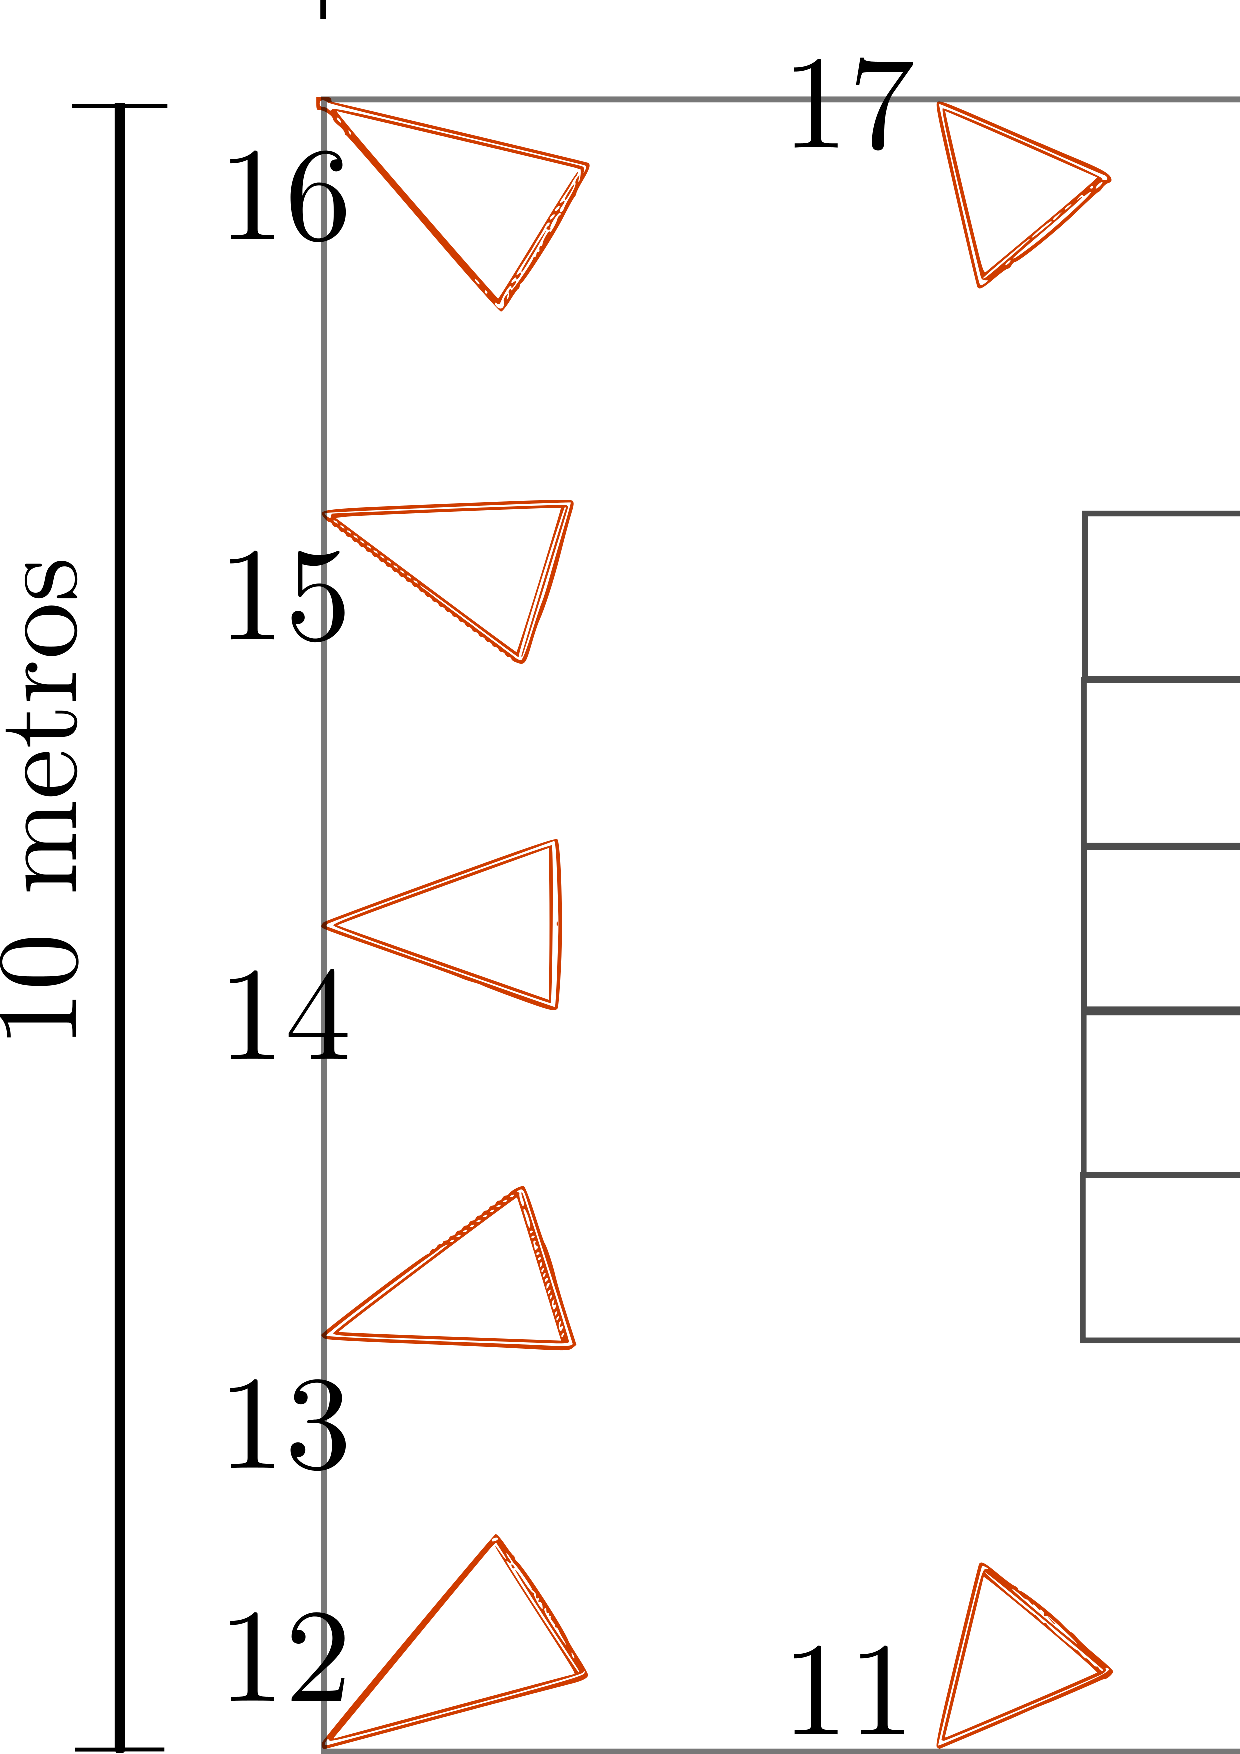
\includegraphics[scale=0.2]{img/Base_Datos/Laboratorio.pdf}}      
  \caption{Toma superior del Laboratorio.\\ Todas las cámaras se encuentran a $1\;m$ del suelo.}
  \label{img_Laboratorio}
\end{figure}  
 
 
\begin{figure}[!ht]
  \centering
   \subfloat[Espacio de captura para marcha rectilínea.]{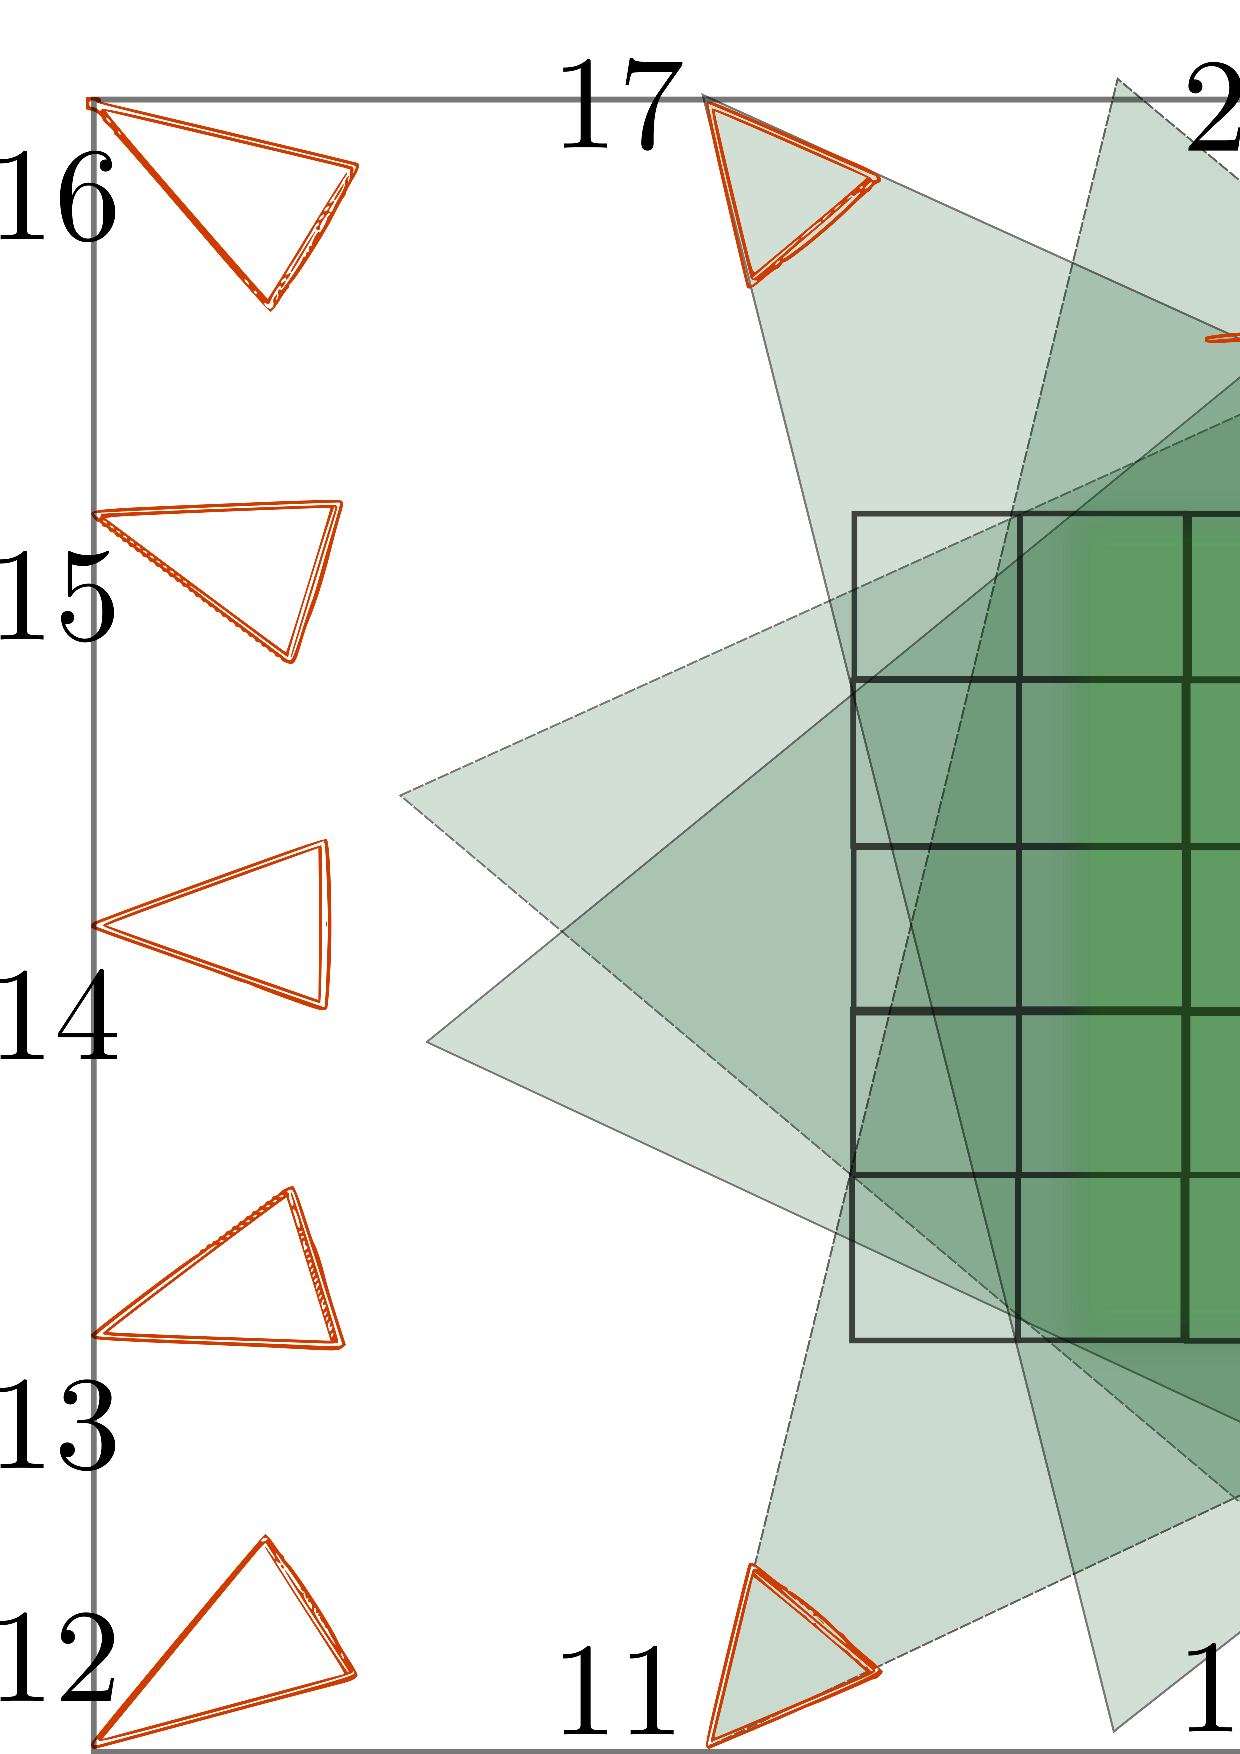
\includegraphics[scale=0.2]{img/Base_Datos/Lab_marcha1.pdf}\label{img_marcha1}}\hspace{0.2cm}
   \subfloat[Espacio de captura para marcha libre.] {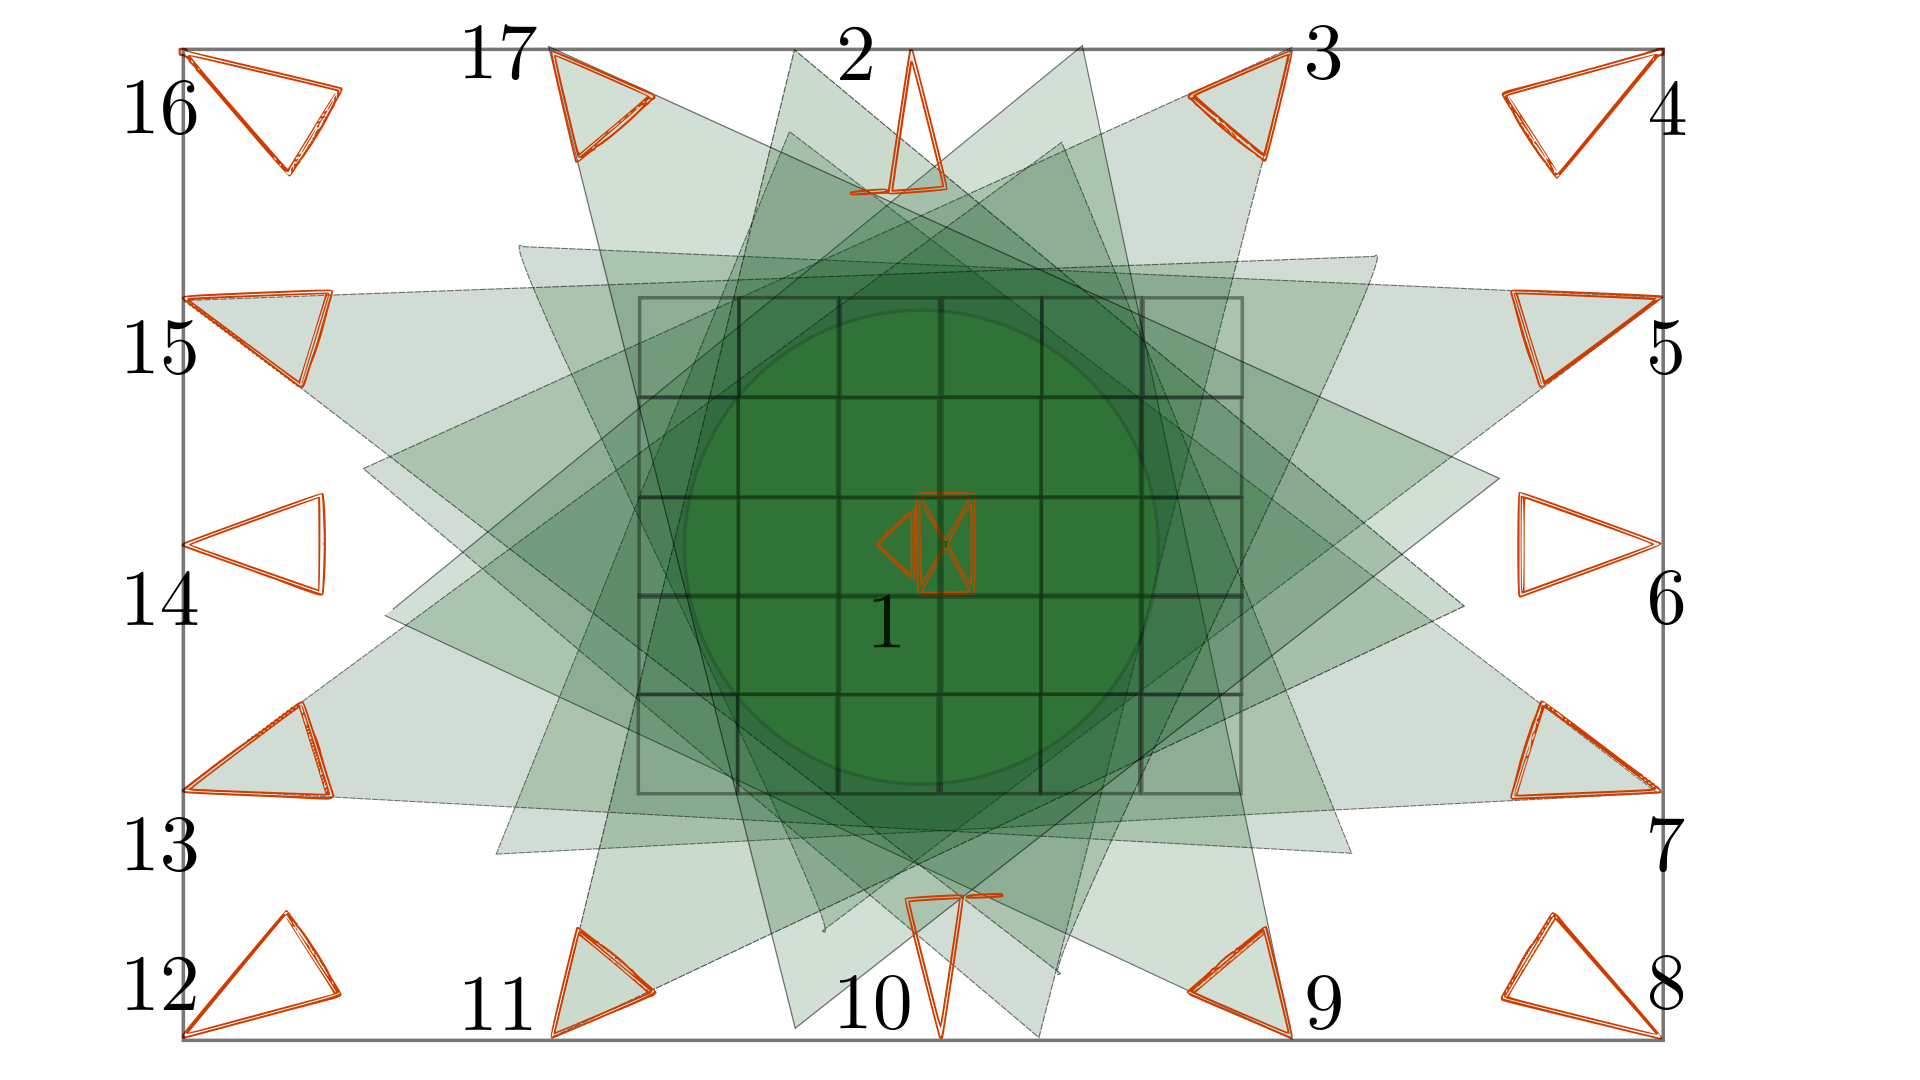
\includegraphics[scale=0.2]{img/Base_Datos/Lab_marcha2.pdf}\label{img_marcha2}}  \caption{Posibles espacios de captura.}
  \label{img_espacio_capura}
\end{figure} 
 
En el caso de la marcha rectilínea puede verse que en principio con tan solo 4 cámaras dispuestas como en la figura \ref{img_marcha1} se genera un espacio de captura útil de aproximadamente $3\;m\times5\; m$ en forma de pasarela. Si el sujeto restringe su movimiento sobre esta zona, dado que la misma se ubica dentro de la intersección de los campos visuales, será visto en su totalidad por todas las cámaras de manera simultánea. En el caso de marcha libre se disponen 8 cámaras intentando que el espacio de captura no tenga direcciones privilegiadas, con lo cual se genera una circunferencia, que en nuestro caso es de aproximadamente $5\;m$ de diámetro. 


Siguiendo el proceso discutido anteriormente \ref{parrafo_Camaras}, se puede estimar la resolución esperada en los datos obtenidos a partir de las secuencias de video, si se cuenta en principio con información de la resolución de las cámaras y su distancia focal. Consideremos nuevamente cámaras con resolución de $1600\times600$ píxeles y distancia focal de $f=32\;mm$, la mayor distancia sobre la cual una cámara debe tener cobertura en la pasarela de la figura \ref{img_marcha1} es de $8 \;m$, mientras que en la figura  \ref{img_marcha2}, caso de la marcha libre, es de $9\;m$, con lo cual un error de un pixel en una cámara produce una incertidumbre de aproximadamente poco más de medio centímetro en ambos casos, a la hora de efectuar la reconstrucción con las secuencias de video obtenidas. 
Debe tenerse presente que estos son casos particulares, pero que permiten hacer una idea de las consideraciones a tener en cuenta para cumplir algunos de los requerimientos del sistema. 
Aumentar el número de cámaras permite una mayor cobertura de volumen, lo que significa una mayor visibilidad del conjunto de marcadores. A su vez una mejor visibilidad del conjunto de marcadores está correlacionado con disminuir la posibilidad de que información importante se pierda en las etapas de análisis de datos posteriores.


\subsubsection{Sincronización} 

Esto resulta esencial en las emisiones con conexiones en directo con varias cámaras, para garantizar que las imágenes de vídeo se mantienen estables incluso cuando se cambia de una cámara a otra.
Se debe contar con un fuente central que envíe una señal de sincronización a todas las videocámaras que participan en una grabación, de esta manera se indica a cada una de ellas cuando deberán comenzar a grabar. 
Esta señal de sincronización puede consistir en eventos sonoros o visuales que permitan sincronizar en etapas de post-procesamiento, pero lo más recomendable si se dispone de equipamiento adecuado es directamente enviar una señal a las cámaras vía hardware.
Si no se contara con una entrada de sincronización sería prácticamente imposible realizar una grabación con varias cámaras simultáneamente.





\subsubsection{Conclusiones} SECCION EN CONSTRUCCION\\
-->especificar los parámetros deseables en una base de datos que trabaje con información óptica basada en marcadores


A la hora de configurar un laboratorio no solo hay que integrar las distintas variables, sino también cuidar que esta integración se gestione de manera compatible, de lo contrario se estaría desaprovechando el potencial de las secuencias generadas por el sistema de captura en cuanto al procesamiento posterior se trata. Dificultando la tarea de obtención de datos a partir de las secuencias de video.

Notar que trabajando a 10 metros con resolución $1600\times600$ se obtienen incertidumbres de pixel de casi $1 ~cm $

\subsection{Base de datos sintética} \label{seccion_Base_Datos_Sintetica}
\subsubsection{Motivación}

No se encontraron base de datos acorde a las necesidades de este proyecto, como se menciona en la sección \ref{conclusiones_revision_base_datos} varios son los motivos, pero básicamente se debe a que ninguna se diseño para el análisis óptico  con marcadores y no ofrecen secuencias de video utilizables para nuestros fines. Por lo tanto se plantea la necesidad de construir una base de datos adecuada que permita desarrollar nuestro sistema.


Una característica importante en muchas de las bases relevadas es la manera con la que habitualmente se obtiene el ground truth a partir de sistemas de captura de movimiento (MoCap), tales como Vicon\footnote{ Sistema  de captura de movimiento (MoCap) de Vicon-Peak, \textcolor{blue}{\underline{\url{http://www.vicon.com/}}} }
 o Impulse\footnote{ Sistema  de captura de movimiento (MoCap) Impulse (PhaseSpace Inc., San Leandro, CA), \textcolor{blue}{\underline{\url{http://www.phasespace.com/}}} },
estos sistemas devuelven información muy precisa sobre la ubicación 3D de marcadores ubicados sobre el sujeto a estudiar. Este tipo de base de datos con capturas de movimiento, se utilizan ampliamente en el ámbito de la animación por computadora, pues se carga la información de la captura al modelo 3D de interés y este efectúa la acción esperada con un alto nivel de realismo. 


Dada la complejidad material y logística de implementar una base de datos, los tiempos necesarios para desarrollar las herramientas de análisis del proyecto y su necesidad de secuencias útiles, junto con el potencial de la información obtenida en el relevamiento de base de datos y sus usos en otros ámbitos, se decide generar una base de datos sintética utilizando el material MoCap utilizado como ground truth.


Continuando en esta dirección al día de hoy, se cuenta con herramientas de código libre para generar una base de datos sintética que sea robusta, completa y extensible. Particularmente se trabajo con la suite de animación 3D Blender\footnote{ Blender Foundation \textcolor{blue}{\underline{\url{http://www.blender.org/}}}}, generando un laboratorio en dicho entorno virtual. Para obtener las secuencias de video, se asocia a un modelo  virtual 3D la información de movimiento de interés obtenida a partir de sistemas MoCap, para luego generar secuencias animadas, las cuales por último se renderizan sobre un cierto número de cámaras para generar secuencias de video conteniendo múltiples vistas del modelo original. Estas secuencias son las que se utilizaron para el desarrollo de nuestro sistema y permitieron generar una base de datos sintética. 


\subsubsection{Formatos Mocap}
La captura de movimiento (Mocap), es una técnica de grabación del movimiento bastante popular en el cual se generan animaciones humanas o animales en ámbitos virtuales a partir de modelos reales. Este tipo de técnicas han sido utilizadas desde hace más de una década en el ámbito del entretenimiento, tales como el cine o los videojuegos e incluso en el ámbito deportivo y médico. 


Importante en la mayoría de las bases de datos relevadas, incluso aquellas de análisis óptico, ya que los sistemas comerciales que efectúan este tipo de capturas devuelven datos con un alto nivel de precisión, por lo que se utilizan como ground truth y se comparan con datos obtenidos a partir de otros sistemas. La primer desventaja de todas estas prestaciones es su alto costo, bastante privativo en muchos ámbitos.

En la actualidad el éxito de las capturas de movimiento ha dado lugar a una serie de casas de producción que pueden registrar y proporcionar datos de movimiento, sin embargo muchas de las empresas han desarrollado su propio formato de archivo. Esto significa que los formatos de archivo de los datos de captura de movimiento
están lejos de unificarse en un estándar, sin embargo la naturaleza ASCII de muchos de los formatos, hace que sea razonablemente fácil decodificar y entender la información por simple inspección de los datos.

\begin{table}[H]
\caption{Formatos de archivo Mocap.}
\label{tabla_Mocap_extensions}
\begin{minipage}{\textwidth}
\centering
\begin{tabular}{|l|l|}
\hline
\textbf{Formatos Mocap} & \multicolumn{1}{c|}{\textbf{Compañia}}                                              \\ \hline
ASF \& AMC              & Acclaim \footnote{\textcolor{blue}{\underline{\url{http://www.darwin3d.com/gamedev/acclaim.zip }}}. Accedido 30-11-14}                                                                            \\ \hline
BVA \& BVH              & BioVision \footnote{\textcolor{blue}{\underline{\url{http://www.biovision.com/bvh.html }}}. Accedido 30-11-14}                                                                          \\ \hline
BRD                     & LambSoft Magnetic Format \footnote{\textcolor{blue}{\underline{\url{http://www.dcs.shef.ac.uk/~mikem/fileformats/brd.html}}}. Accedido 30-11-14}                                                           \\ \hline
C3D                     & \begin{tabular}[c]{@{}l@{}}Biomechanics, Animation and\\ Gait Analysis \footnote{\textcolor{blue}{\underline{\url{http://www.c3d.org/c3d_format.htm }}}. Accedido 30-11-14}\end{tabular} \\ \hline
CSM                     & \begin{tabular}[c]{@{}l@{}}3D Studio Max, \\ Character Studio\footnote{\textcolor{blue}{\underline{\url{http://www.dcs.shef.ac.uk/~mikem/fileformats/csm.html}}}. Accedido 30-11-14}\end{tabular}          \\ \hline
GTR, HTR \& TRC         & Motion Analysis \footnote{\textcolor{blue}{\underline{\url{http://research.cs.wisc.edu/graphics/Courses/cs-838-1999/Jeff/MoCapTOC.html}}}. Accedido 30-11-14}                                                                    \\ \hline
\end{tabular}
\end{minipage}
\end{table}
La aplicación que se realice condiciona cual de los formatos de la tabla \ref{tabla_Mocap_extensions} es más conveniente. 
La mayoría de los formatos mostrados son soportados por Blender, sin embargo dado que nuestro interés es la manipulación y fácil interpretación de la información, el formato elegido para manipular las capturas de movimientos es el BVH, por ser posiblemente el más compacto, conciso y ampliamente utilizado. De todas maneras se cuenta con funciones en Matlab para llevar la información de movimiento contenida en estos archivos a varios de los formatos descriptos en la tabla \ref{tabla_Mocap_extensions}, así como también directamente a una matriz con las coordenadas 3D de cada marcador a lo largo del tiempo.

\paragraph{BVH (BioVision Hierarchical data )}

El formato BVH proviene del formato BVA de BioVision con la notable adición de una estructura de datos jerárquica que representa los huesos\footnote{Entidad básica en la representación del esqueleto. Cada hueso representa el segmento más pequeña dentro del movimiento sujeto a cambios de traslación y rotación. } del esqueleto\footnote{Entidad global que representa el movimiento. Un esqueleto está formado por huesos.}. Se compone de dos partes, la primera sección detalla la jerarquía y la pose inicial del esqueleto y la segunda sección el movimiento del mismo, describiendo la información temporal del esqueleto cuadro a cuadro.
 
 
\begin{figure}[!ht]
  \centering 
   \subfloat[Esqueleto]{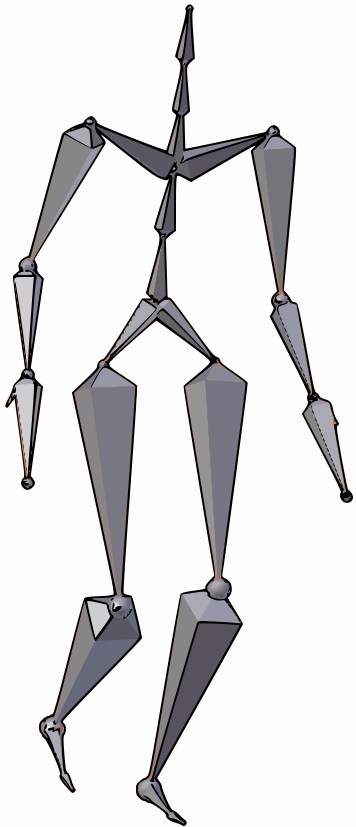
\includegraphics[scale=0.25]{img/Base_Datos/Estructura_esqueleto1.pdf}\label{img_Esqueleto_1}}
   \subfloat[Estructura jerárquica]{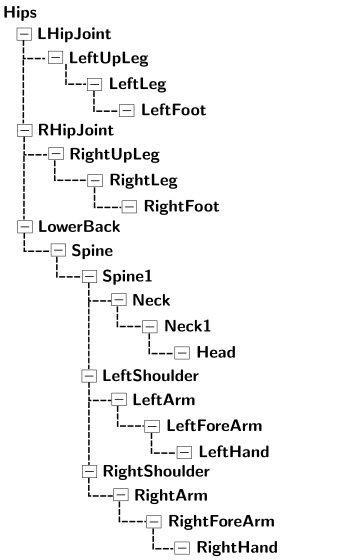
\includegraphics[scale=0.4]{img/Base_Datos/Estructura_bvh.png}\label{img_estructura_bvh}}\hspace{0.1cm}   
   \subfloat[Sección de jerarquía]{\includegraphics[scale=0.2]{img/Base_Datos/BVH_Encabezado.png}\label{img_BVH_Encabezado}}\hspace{0.01cm}   
   \subfloat[Sección de movimiento]{\includegraphics[scale=0.2]{img/Base_Datos/BVH_Motion.png}\label{img_BVH_Motion}}  
   \caption{Información contenida en archivos BVH.}  
\end{figure}   

La sección jerárquica del archivo empieza con las dos primeras líneas conteniendo las palabras HIERARCHY y ROOT respectivamente, seguidas del nombre del hueso que es la raíz de la estructura jerárquica y a continuación la estructura restante del esqueleto definida de manera recursiva conteniendo la información del origen de cada hueso y el orden en que las variables del hueso se modifican en la segunda sección. La sección de movimiento empieza con la palabra clave MOTION, contiene la cantidad de cuadros en la secuencia, el tiempo entre cuadros y la  información completa de la posición de cada hueso del esqueleto en cada cuadro de la secuencia. Por más detalles del formato consultar el artículo de M. Meredith y S.Maddock \cite{meredith2001motion}.  

Si bien en principio cualquier fuente de archivos BVH con capturas de movimiento es válida, se decide trabajar en este proyecto con las fuentes BVH de la base de datos \textit{MotionBuilder-friendly version} ofrecidas por cgspeed\footnote{\textcolor{blue}{\underline{\url{https://sites.google.com/a/cgspeed.com/cgspeed/motion-capture}}}. Accedido 4-12-14},
 que provienen de las capturas de Carnegie Mellon University Motion Capture Database\footnote{\textcolor{blue}{\underline{\url{http://mocap.cs.cmu.edu/}}}. Accedido 30-11-14}. 
 Como se menciona anteriormente en la sección \ref{CMU}, CMU dispone de un gran número de capturas de movimiento de acceso público, varias utilidades de software que permiten llevar a otros formatos y es utilizado ampliamente en el ámbito de la animación por computadora.




\subsubsection{Blender} %SECCION EN CONSTRUCCION\\
En esta sección se describe de que manera se utiliza Blender y Python para generar las secuencias de video de la base de datos. Los parámetros de las distintas componentes así como los detalles de procesos enumerados en esta sección se encuentran en el apéndice (COLOCAR AQUI LA REFERENCIA PARA EL APENDICE).



Blender es una suite de animación 3D gratuita y de código abierto, la misma cuenta con las herramientas necesarias para trabajar en todas las etapas de desarrollo de un proyecto de animación 3D. Por otro lado posee una interfaz de programación de aplicaciones muy fexible y potente que permite extender su funcionalidad a través de programas en lenguaje Python. Estas cualidades son muy útiles para generar nuestra base de datos por lo que se decidió desarrollar la misma utilizando las herramienta de esta aplicación.

Se ha generado un espacio de trabajo controlado, conteniendo entre otras cosas un cierto número de cámaras, iluminación, color de fondo determinado y un modelo con marcadores sobre el cual cargar la captura de movimiento de interés. También se han implementado programas en Python para facilitar múltiples tareas:

\begin{itemize}
\item  ayudar en  el ajuste de las capturas provenientes de archivos BVH al esqueleto del modelo virtual,
\item	generar las secuencias de video a partir de archivos .blend  con el modelo virtual desarrollando el movimiento de interés,
\item	exportar la información de calibración de las cámaras en un archivo .m para usar la misma desde Matlab.
\end{itemize}


\begin{figure}[!ht]
  \centering 
   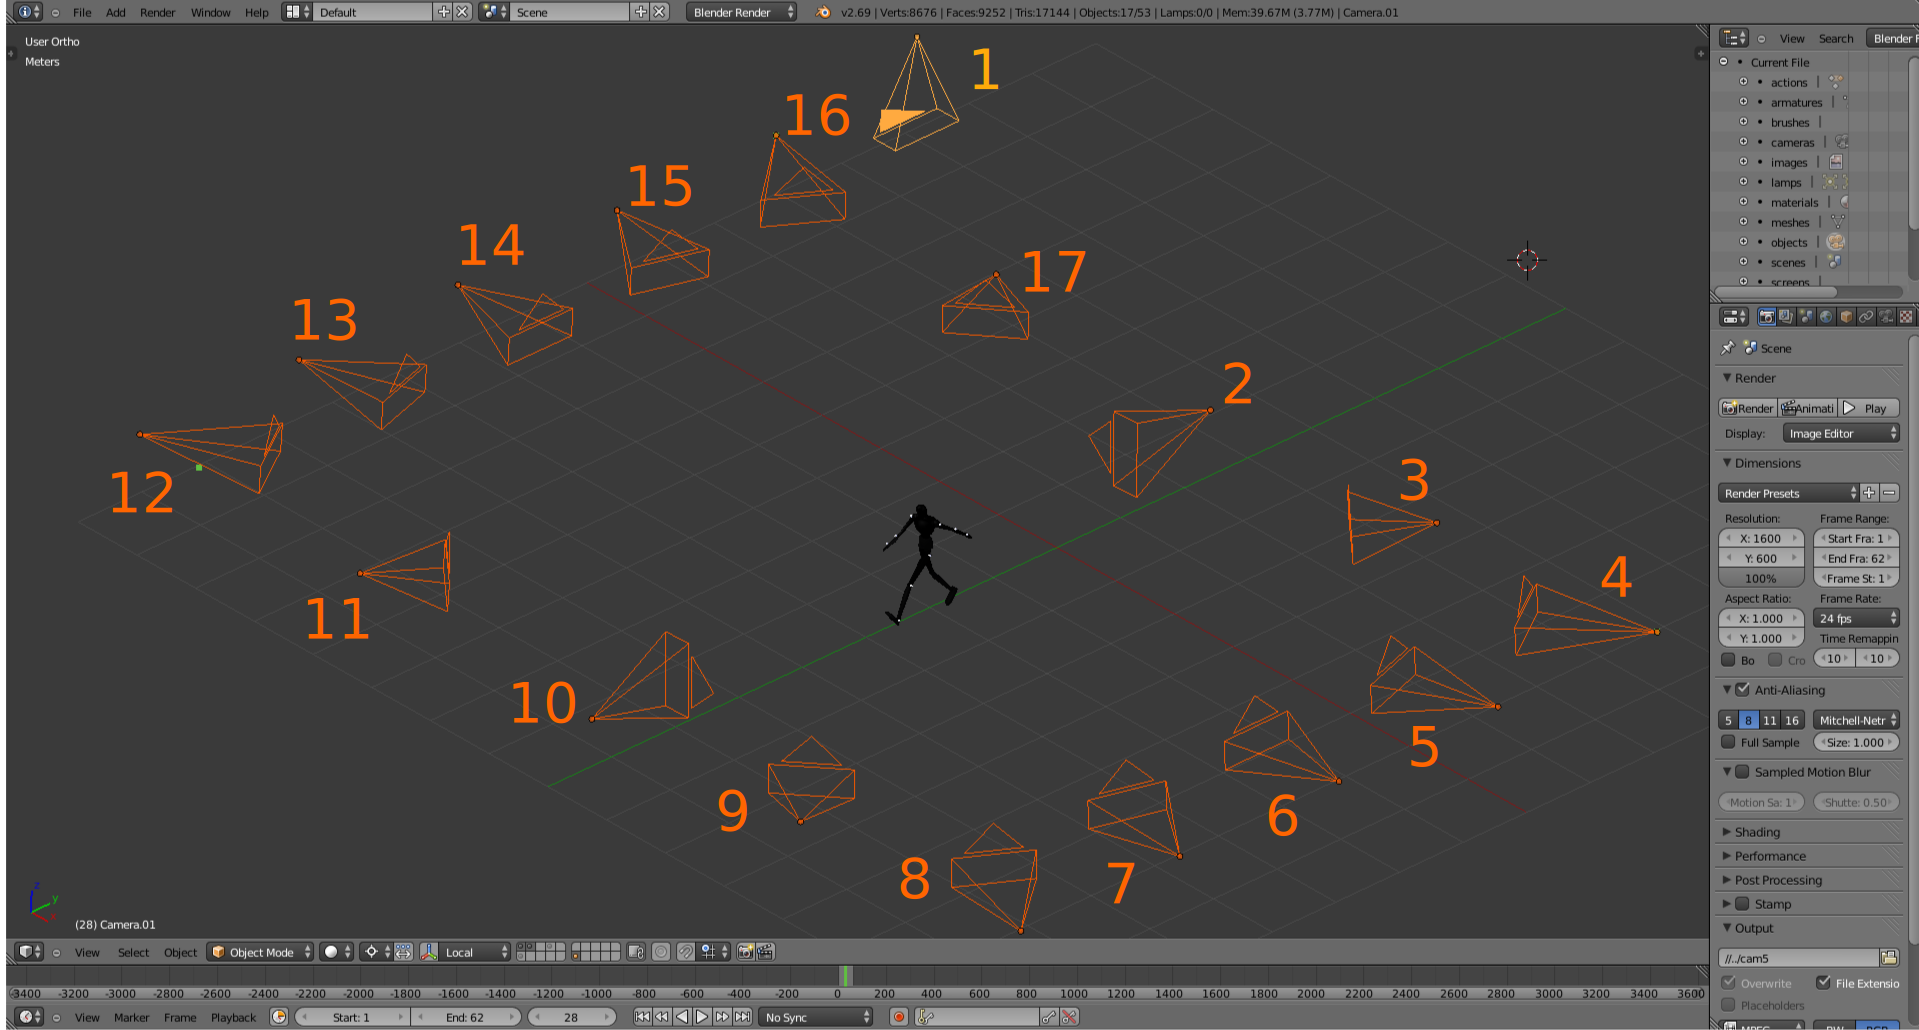
\includegraphics[scale=0.3]{img/Base_Datos/Entorno_Blender.pdf}
   \caption{Entorno de trabajo en Blender.}
  \label{img_Entorno_Blender}
\end{figure}   


\paragraph{Disposición del laboratorio}
El laboratorio generado posee 17 cámaras dispuestas en un ambiente rectangular de $10\times15\;m $ como se muestran en las figuras \ref{img_Laboratorio} y \ref{img_Entorno_Blender}. La configuración de las mismas permite probar diferentes combinaciones de captura a la hora de generar secuencias. Se diseñaron las cámaras para que sus parámetros fuesen similares a cámaras convencionales
 encontradas en el mercado y utilizadas en las bases de datos relevadas. 
 Las posiciones y valores característicos de las cámaras pueden verse en detalle en el apéndice  
 (PONER AQUI LA REFERNECIA AL APENDICE DONDE SE MUESTRA LA SALIDA DE INFOCAMBLENDER). Para iluminar el laboratorio se dispusieron $8$ focos puntuales de luz omnidireccional sobres los límites del mismo, rodeando la escena y a un nivel de 3 metros de altura. De esta manera se garantiza que ninguno de los focos sea tomado directamente por las cámaras y los marcadores se iluminan correctamente.
 

\paragraph{Modelo virtual}  
El modelo virtual utilizado se basa en un maniquí de madera convencional, la elección del mismo responde a la facilidad con la que se puede ajustar el mismo a una posición particular, siendo cada miembro fácilmente correlacionado con un hueso específico, sin perder las particularidades propia de un sujeto real. Cabe destacar que la relevancia del modelo en las capturas es simular las oclusiones de marcadores debida a los miembros del sujeto en una captura real.  

Para la elección del material aplicado al modelo virtual, se toman en cuenta las consideraciones planteadas en la sección \ref{seccion_Caracteristicas_Laboratorio}, dado que los marcadores que se van a utilizar son de color difuso blanco, se decide aplicar sobre el modelo un material difuso negro con especularidad baja, de manera que no se generen brillos indeseados debido a la iluminación en el momento de la captura. De esta manera la configuración recomendada es utilizar un fondo también oscuro.

\paragraph{Esqueleto}
En cuanto a el esqueleto con la información de movimiento, el mismo se obtuvo de la base de datos \textit{MotionBuilder-friendly version} (de aquí en más MotionBuilder) ofrecidas por cgspeed\footnote{\textcolor{blue}{\underline{\url{https://sites.google.com/a/cgspeed.com/cgspeed/motion-capture}}}. Accedido 4-12-14},
 donde se cuenta con las fuentes BVH que provienen de las capturas de movimiento de CMU (sección \ref{CMU}). Si bien cgspeed ofrece otras bases más nuevas, donde la jerarquía del esqueleto en los archivos BVH a sido reducida con el fin de facilitar el ajuste a modelos virtuales, se ha trabajado con la base original antes mencionada. Aparentemente el procesamiento aplicado para producir las nuevas bases, introdujo ruido sobre algunos cuadros en las secuencias originales, esto se a constatado al importar en Blender dichas secuencias.
      
 Con el fin de normalizar las secuencias BVH provenientes de MotionBuilder se a utilizado la herramienta de edición de archivos BVH bvhacker\footnote{bvhacker: The free bvh file editing tool. \textcolor{blue}{\underline{\url{ http://davedub.co.uk/bvhacker/}}}. Accedido 5-12-14}. La misma permite centrar las secuencias sobre un mismo punto en el primer frame  removiendo los offset globales.
 Una vez gestionado lo anterior se importa en Blender la secuencia BVH y se procede a generar los marcadores en las articulaciones del esqueleto, dado que se tiene la posición exacta del origen de cada hueso en el esqueleto y la articulación es la unión entre dos huesos consecutivos, se puede obtener la posición exacta de los marcadores a partir de la secuencia BVH.
 La generación de los marcadores y el enlazado del esqueleto al modelo se realiza a través de un código python, \texttt{acoplar\_modelo.py}, realizado para tal fin. El mismo genera marcadores esféricos de material difuso blanco levemente poroso, con $2,8 \;cm$ de diámetro y baja especularidad, centrados en las articulaciones definidas previamente en una lista, como se muestra en la figura \ref{img_esqueleto_marcador} y luego enlaza cada miembro del modelo a su correspondiente hueso. De está manera para finalizar la creación del modelo con marcadores solo resta que el usuario realice ajuste mínimos de tamaño y posición sobre el modelo. Es importante resaltar que los marcadores se ubican sobre puntos del esqueleto de los cuales se conoce la posición 3D en cada cuadro. y que el modelo es necesario debido a que el esqueleto no se puede renderizar. 
 
 \begin{figure}[H]
   \centering 
   \subfloat[Creación de marcadores]{\includegraphics[scale=0.25]{img/Base_Datos/Esqueleto_Marcador.pdf}\label{img_esqueleto_marcador}} \hspace{0.6cm}
   \subfloat[Ajuste de modelo]{\includegraphics[scale=0.25]{img/Base_Datos/Modelo_Marcador.pdf}\label{img_modelo_marcador}}
   \caption{Generación de marcadores sobre el modelo virtual.}   
 \end{figure}  
 
Una ves finalizado el proceso, figura \ref{img_modelo_marcador},  el modelo puede realizar el movimiento contenido en la secuencia BVH y solo resta renderizar. 

\paragraph{Renderizado} 

Ya se dispone de la secuencia de movimiento en el entorno virtual de Blender, lo que resta es renderizar dicha secuencia sobre las cámaras del laboratorio. Para ello se implementó un código en python, \texttt{render.py},  que automatiza todo el proceso, dispone los videos obtenidos en cada render con nombres y ubicaciones predefinidas en la base de datos y genera un código Matlab con la información ground truth de cada cámara. 


 \begin{figure}[H]
   \centering 
   \subfloat[Importación de secuencia BVH y generación de marcadores]{\includegraphics[scale=0.25]{img/Base_Datos/Esqueleto_Render.pdf}} \hspace{1.0cm}
   \subfloat[Modelo enlazado al esqueleto]{\includegraphics[scale=0.25]{img/Base_Datos/Modelo_Render.pdf}}
   \hspace{1.3cm}
   \subfloat[Imagen renderizada]{\includegraphics[scale=0.205]{img/Base_Datos/Modelo_Render2.png}}
   \caption{Creación de secuencias en Blender.}   
 \end{figure} 


 
\paragraph{Ground truth} 

Para contar con el ground truth final de la secuencia animada se debe exportar desde Blender la información del esqueleto en un BVH, cuidando que se mantenga la misma escala de tiempos que en el momento del renderizado. De esta manera se tienen sincronizados los videos y el ground truth 3D.

\paragraph{Mocap Tools}

Existe una herramienta en Blender que permite manipular y copiar la información de movimiento entre dos esqueletos, denominada \textit{Mocap Tools} . La misma no viene activada por defecto y se debe habilitar desde el menú de preferencias. Para la creación de secuencias utilizando esta herramienta, se debe tener un esqueleto ya enlazado al modelo virtual con marcadores, luego se importa la secuencia BVH de interés que a su vez genera otro esqueleto. Utilizando las opciones de \textit{Mocap Tools}  se copia el movimiento del esqueleto BVH al esqueleto ya definido inicialmente, de esta manera se evitan los ajustes posteriores del modelo virtual y se tiene una secuencia lista para renderizar. 
El problema surge al momento de obtener el ground truth, pues la exportación del esqueleto que se utiliza para mover al modelo no es precisa en este caso, se detectaron fallas en este sentido por parte de Blender, solo se exportan los movimientos relativos de los huesos y no la traslación del centro de masa del esqueleto. El motivo fundamental es el mecanismo utilizado por \textit{Mocap Tools} para enlazar los dos esqueletos, el BVH y el del modelo virtual. Dado que la información de traslación no se incluye en el esqueleto de destino sino que se condiciona a que este último se traslade según un hueso particular externo (\textsf{stride bone})  cuya información de movimiento no puede ser exportada en un BVH por Blender. Con lo cual, si bien al trabajar con esta herramienta se generan secuencias visualmente aceptables para un proceso de animación, en nuestro caso impide obtener el ground truth necesario para las etapas de performance y desarrollo, por lo que no se utiliza.
 
    


%Describir como está armado el laboratorio (meter dos fotos una con las cámaras numeradas, otra con el entorno blender y el macaco). Explicar en que layers se dejan las cámaras\\
%Describir como está armado el macaco, que colores se le pusieron, etc.\\
%Describir como se importa un esqueleto al blender. Pasos previos, uso del programa bvhacker\\
%Describir como se generan los marcadores y se ajusta el esqueleto. Explicar que como lo que se conoce son las posiciones de las intersecciones entre huesos del esqueleto se debe ajustar el modelo Blender de manera especial y poner los marcadores sobre dichas intersecciones.\\
%Informar sobre el problema que se encontró al utilizar el programa de ajuste de esqueleto.\\
%Exportación del ground truth desde Blender.\\




\subsubsection{Estructura de la base de datos}

El prototipo de base de datos, actualmente contiene 5 secuencias sintéticas descriptas en la tabla \ref{tabla_secuencias_gen}, las mismas fueron generadas a partir de las secuencias BVH provenientes la 
base de datos \textit{MotionBuilder-friendly version} ofrecidas por cgspeed\cite{cgspeed}, cuyo origen son las capturas de movimiento de CMU (sección \ref{CMU}). 


%Describir el tipo de información,como está guardada y como se gestiona.\\
%Introducción de nuevas secuencias\\
%Programas Python utilizados y exportaciones a otras formatos\\



\begin{table}[h!]
\centering
\caption{Secuencias generadas para la base de datos sintética.}
\label{tabla_secuencias_gen}
\begin{tabular}{|l|c|r|r|r|}
\hline
\multicolumn{1}{|c|}{\textbf{Acción}}                                            & \textbf{\begin{tabular}[c]{@{}c@{}}Nro. de\\ secuencia\\ CMU\end{tabular}} & \textbf{\begin{tabular}[c]{@{}c@{}}Longitud \\ de secuencia\\ (segundos)\end{tabular}} & \textbf{\begin{tabular}[c]{@{}c@{}}Cuadros por\\ segundo\end{tabular}} & \textbf{\begin{tabular}[c]{@{}c@{}}Espacio \\de captura\\ (metros)\end{tabular}} \\ \hline
Marcha rectilínea                                                                & 08\_03                     & 2.5                                                                                    & 30                           & 1,5$\times$ 5,5                                                                            \\ \hline
\begin{tabular}[c]{@{}l@{}}Marcha rectilínea, \\ zancada exagerada\end{tabular}  & 08\_07                     & 2.6                                                                                    & 24 y 48                      & 1,5$\times $5,5                                                                            \\ \hline
\begin{tabular}[c]{@{}l@{}}Marcha rectilínea\\ lenta, zancada ancha\end{tabular} & 08\_11                     & 3.8                                                                                    & 30                           &1,5$\times $5                                                                            \\ \hline
Corriendo                                                                        & 09\_07                     & 1.2                                                                                    & 24 y 48                      &1,5$\times $5                                                                              \\ \hline
Marcha libre                                                                     & 09\_12                     & 12.5                                                                                   & 24                           &3$\times $5                                                                              \\ \hline
\end{tabular}
\end{table}


La estructura utilizada para los directorios de la base de datos es la siguiente:
\begin{description}
\item[{\small\textbf{\textsf{<Sujeto>/<Nro\_Secuencia>/Datos\_Imagen/}}}] \hfill \\
Contiene los datos de videos de las secuencias de movimiento.\vspace{-0.2cm}
	\begin{description}
	\item[{\small\textbf{\textsf{cam<nro\_cámara>.dvd}}}] - nombre de los videos con compresión mpeg.
	\end{description} 
	% % % % % % % % % % % % % % % % % % % % % % % % %
\item[{\small\textbf{\textsf{<Sujeto>/<Nro\_Secuencia>/Ground\_Truth/}}}] \hfill \\
Contiene tres carpetas con el ground truth de cada sección del sistema de procesamiento. \vspace{-0.2cm}
	\begin{description}
	\item[{\small\textbf{\textsf{Deteccion/}}}] \hfill \\\vspace{-0.5cm}
		\begin{description}
			\item[{\small\textbf{\textsf{cam.xml}}}] - archivo con la información de posición 2D de los marcadores sobre cada retina obtenida a partir de los ground truth de posición 3D y calibración. La información se dispone como se indica en la estructura de datos de la sección \ref{section_Estructura_de_datos}.   
			\item[{\small\textbf{\textsf{cam.mat}}}] - posee la misma información que {\small\textbf{\textsf{cam.xml}}} pero contenida en una variable matlab.
		\end{description} 			
	\item[{\small\textbf{\textsf{Reconstruccion}}}/] \hfill \\ \vspace{-0.5cm}		
		\begin{description}
			\item[{\small\textbf{\textsf{skeleton.xml}}}] -  archivo que contiene la posición 3D de los marcadores. La información se dispone como se indica en la estructura de datos de la sección \ref{section_Estructura_de_datos}.   
			\item[{\small\textbf{\textsf{skeleton.mat}}}] -  posee la misma información que {\small\textbf{\textsf{skeleton.xml}}} pero contenida en una variable matlab.
		\end{description}
	\item[{\small\textbf{\textsf{Seguimiento}}}/] \hfill \\ \vspace{-0.5cm}
		\begin{description}
				\item[{\small\textbf{\textsf{skeleton.xml}}}] - archivo que contiene las trayectorias 3D de los marcadores. La información se dispone como se indica en la estructura de datos de la sección \ref{section_Estructura_de_datos}.   
				\item[{\small\textbf{\textsf{skeleton.mat}}}] -  posee la misma información que {\small\textbf{\textsf{skeleton.xml}}} pero contenida en una variable matlab.
		\end{description}
	\end{description}
% % % % % % % % % % % % % % % % % % % % % % %	
\item[{\small\textbf{\textsf{<Sujeto>/<Nro\_Secuencia>/Datos\_Procesados/}}}] \hfill \\
Contiene tres carpetas con la información de cada sección del sistema de procesamiento. \vspace{-0.2cm}
	\begin{description}
	\item[{\small\textbf{\textsf{Deteccion}}}/] \hfill \\\vspace{-0.5cm}
		\begin{description}			
			\item[{\small\textbf{\textsf{cam.xml}}}] - archivo con la información de posición 2D de los marcadores sobre cada retina obtenida a partir del bloque de detección de marcadores. La información se dispone como se indica en la estructura de datos de la sección \ref{section_Estructura_de_datos}. La calibración es del ground truth.  
			\item[{\small\textbf{\textsf{cam.mat}}}] - posee la misma información que {\small\textbf{\textsf{cam.xml}}} pero contenida en una variable matlab.
		\end{description} 			
	\item[{\small\textbf{\textsf{Reconstruccion}}}/] \hfill \\ \vspace{-0.5cm}		
		\begin{description}
			\item[{\small\textbf{\textsf{skeleton.xml}}}] -  archivo que contiene la posición 3D de los marcadores obtenida a la salida del bloque de reconstrucción. La información se dispone como se indica en la estructura de datos de la sección \ref{section_Estructura_de_datos}.
			\item[{\small\textbf{\textsf{skeleton.mat}}}] - posee la misma información que {\small\textbf{\textsf{skeleton.xml}}} pero contenida en una variable matlab.
		\end{description}
	\item[{\small\textbf{\textsf{Seguimiento}}}/] \hfill \\ \vspace{-0.5cm}
		\begin{description}
				\item[{\small\textbf{\textsf{skeleton.xml}}}] - archivo que contiene las trayectorias 3D de los marcadores obtenida a partir del bloque de seguimiento. La información se dispone como se indica en la estructura de datos de la sección \ref{section_Estructura_de_datos}. 
				\item[{\small\textbf{\textsf{skeleton.mat}}}] - posee la misma información que {\small\textbf{\textsf{skeleton.xml}}} pero contenida en una variable matlab.
		\end{description}
	\end{description}
% % % % % % % % % % % % % % % % % % % % % % %
\item[{\small\textbf{\textsf{Calibracion/Datos\_Imagen}}}] \hfill \\
VER CON GUILLERMO CUANTAS FORMAS DE CALIBRAR TENEMOS \vspace{-0.2cm}
\item[{\small\textbf{\textsf{Calibracion/Ground\_Truth}}}] 
\item[{\small\textbf{\textsf{Calibracion/Datos\_Procesados}}}] 
\end{description}
% % % % % % % % % % % % % % % % % % % % % %
% % % % % % % % % % % % % % % % % % % % % %

Dentro de cada <...>  ~designar el nombre de la variable que se indica.


\subsubsection{Estructura de datos.}
\label{section_Estructura_de_datos}
Para poder trabajar a lo largo de todo el sistema de procesamiento se debe contar con una estructura de datos que mantenga y soporte toda la información de interés a lo largo proceso. También es deseable que los procesos utilicen dicha estructura sin quedar condicionados a futuras modificaciones de la misma, esta independencia requiere la existencia de funciones de acceso de entrada y salida a la estructura.  


Con este fin se ha diseñado e implementado las estructuras de datos de las figuras \ref{img_estructura_skeleton} y \ref{img_estructura_cam}.
Las mismas permiten almacenar tanto la información de ground truth como la generada a la hora de  trabajar en las etapas de análisis de video. Se han implementado funciones de acceso de entrada y salida en Matlab, así como varias herramientas de gestión. Que permiten entre otras cosas inicializar las estructuras, obtener o modificar cualquier parámetro, efect 


exportación e importación a xml, 


Básicamente se tienen dos estructuras principales, una para almacenar información del esqueleto asociado al modelo y otra para almacenar la información de las cámaras con las que se efectúa la captura de video.

Cabe destacar que este tipo de estructura es útil tanto para una base de datos sintética como una base de datos real. \\
\\

\begin{figure}[H]
   \centering 
   \includegraphics[scale=0.6]{img/Base_Datos/Estructura_datos_skeleton.pdf}
   \caption{Estructura de datos para esqueletos.}  
   \label{img_estructura_skeleton} 
 \end{figure} 

\begin{figure}[H]
   \centering 
   \includegraphics[scale=0.6]{img/Base_Datos/Estructura_datos_cam.pdf}
   \caption{Estructura de datos para cámaras.}
   \label{img_estructura_cam}    
 \end{figure} 

Porque se necesita\\
Que forma tiene\\
Cual es su alcance\\
Como se gestiona (tengo que hablar de las funciones que manejan la base de datos, al menos globalmente que se puede hacer....ufffffff
, acordarse que están diseñadas para una fácil exportación a xml)\\
\\
\subsubsection{Conclusiones} SECCION EN CONSTRUCCION\\
sobre como quedo la base de datos, utilidad, potencial y posible expansión




MATERIAL PARA RECICLAR\\


Si bien las secuencias de video obtenidas son lo único necesario para el análisis de video, al generar dichas secuencias a través de un entorno virtual controlado, se puede obtener la información exacta del ambiente de captura. Información de las cámaras, iluminación, colores, ruido, posición de los marcadores en cada frame, etc. Permitiendo contar con un ground truth sobre el cual validar los algoritmos de análisis de video. 

Dado que Blender se encuentra implementado sobre Python, se ha creado un script que permite una vez generada la secuencia, automatizar la extracción de estos parámetros de interés hacía un archivo xml con cierta estructura particular ya definida en la base de datos. 
 


\subsection{Conclusiones} SECCION EN CONSTRUCCION\\
sobre todo el capitulo, resumen de conclusiones parciales



\clearpage
\section{Implementación de bloques del sistema}
%%%%%%%%%%%%%%%%%%%%%%%%%%%%%%%%%%%%%%%%%%%%%%%%%%%%%%%%%%%%%%%%%%%%%%%%%%%5%%%%%%%%%%%%%%%%%%%%%%%%%%%%%%%%%%%%%%%%%%%%%%%%%%%%%
%por qué este algoritmo? cómo se hace? explicar la filosofía de conseguir una implementación y adaptarla a nuestro propósito, y que la realidad es que no hay muchos sistemas disponibles. La justificacion puede venir por dos ejes: complejidad del algoritmo, en uruguay no hay casi experiencia industrial en procesamiento de imagenes. por qué no se usó un detector de circulos? son cosas muy chicas y en realidad no son circulos perfectos. La explicación del algoritmo tiene que ser bien detallada. En qué lenguaje se programó, justificar herramientas (por qué opencv, por qué c++, etc.)
%%%%%%%%%%%%%%%%%%%%%%%%%%%%%%%%%%%%%%%%%%%%%%%%%%%%%%%%%%%%%%%%%%%%%%%%%%%%%%%%%%%%%%%%%%%%%%%%%%%%%%%%%%%%%%%%%%%%%%%%%%%%%%%%%%

%COMENTARIO: ACÁ SE ME OCURRE DE HACER UNA INTRODUCCIÓN A CADA BLOQUE DEL SISTEMA, JUSTIFICAR Y EXPLICAR MEDIO POR ARRIOBA Y EN LAS SIGUIENTES SECCIONES EXPLICAR LOS DETALLES MÁS TÉCNICOS DE CADA BLOQUE.
\clearpage
\section{Segmentación}
%pag 711, Gonzalez 3º ed

\subsection{Introducción}

El término segmentar hace referencia, en rasgos generales, a la división de una imagen en múltiples secciones u objetos para su posterior análisis. En otras palabras, la segmentación se encarga de identificar los objetos de importancia dentro de la imagen, en este caso los marcadores. El nivel de detalle de esta división depende del problema a atacar.

Este proceso es uno de los más importantes dentro de un sistema de captura de movimiento ya que en base a los datos obtenidos aqui, se realizará tanto el tracking como la reconstrucción 3D por lo que un error en la detección de la posición de los marcadores será imposible de detectar en etapas posteriores y generará un seguimiento 3D erróneo del mismo. Más aun si se tiene en cuenta que el sistema será aplicado para la medicina, por lo que deberá tener una exactitud mayor que otros sistemas donde la precisión no juega un papel tan importante (como el Kinect de Microsoft\cite{kinect} por ejemplo).

Existen varios métodos a aplicar para realizar la segmentación, en esta sección se describirán los tipos más importantes asi como la elección realizada para la implementación de este sistema, además se explicará como funciona el bloque desarrollado.

\subsection{Estado del arte}

Para realizar la segmentación existen varios métodos, los algoritmos para tratar imagenes monocromáticas generalmente se clasifican en dos grupos basados en la intensidad de los pixeles: discontinuidad y similaridad. 

En los algoritmos basados en discontinuidad, se parte de la suposición que los límites de las regiones son suficientemente distintos unos de otros y del fondo para permitir detectarlos en base a las discontinuidades de intensidad. Los algoritmos principales en esta categoría son los basados en \textbf{detección de bordes}.

Por otro lado, en los algoritmos basados en similaridad, se busca dividir la imagen en diferentes zonas donde los pixeles de cada una son similares entre si y comparten ciertas características predefinidas. Los algoritmos más conocidos son los basados en identificación de regiones, como por ejemplo la \textbf{aplicación de umbral}.

A continuación se explican los algoritmos mencionados que, como se dijo, son dos de los más importantes dentro de la segmentación.

\subsubsection{Detección de bordes}
\label{detecbordeSec}

De los dos métodos nombrados anteriormente, este es el más complejo y pesado operacionalmente. Básicamente se trata de la detección de líneas o transiciones en una imágen mediante el procesamiento de los pixeles que la componen. A continuación se explica el detalle de este método, como se menciona en el libro \textit{Digital Image Processing de Rafael Gonzalez y Richard Woods}\cite{Gonzalez}.

Asi como el difuminado en una imagen (que equivale a hacer un promedio de los pixeles en una zona) puede realizarse mediante la integración, los cambios de intensidad abruptos entre pixeles continuos pueden detectarse utilizando derivadas. Por razones que serán evidentes más adelante, las derivadas de primer y segundo orden son particularmente las más indicadas para este propósito.

Las derivadas de una función digital son siempre definidas en términos de diferencia. Hay varias formas de aproximar estas diferencias pero para lograr detectar bordes de forma correcta es necesario que la aproximación usada para la derivada de primer orden:

\begin{enumerate}
\item valga cero en áreas de intensidad constante
\item no valga cero al inicio de un escalón o rampa de intensidad
\item no valga cero en los puntos pertenecientes a una rampa de intensidad
\end{enumerate}

De la misma forma, se requiere que la aproximación utilizada para la derivada de segundo orden:

\begin{enumerate}
\item valga cero en áreas de intensidad constante
\item no valga cero al inicio y al final de un escalón o rampa de intensidad
\item no valga cero en los puntos pertenecientes a una rampa de intensidad
\end{enumerate}

Utilizando la definición de derivada desde el punto de vista del cálculo funcional, y simplificando por el desarrollo de Taylor de primer grado alrededor del punto $x$, considerando una variación de $\partial x$ unitaria, se obtiene:
\begin{equation}
\frac{\partial f}{\partial x} = f'(x) = f(x+1)-f(x)
\label{derivada1}
\end{equation}

análogamente, para la derivada segunda:

\begin{equation}
\frac{\partial^2 f}{\partial x^2} = f''(x) = f(x+1)-f(x-1)-2f(x)
\label{derivada2}
\end{equation}

Se puede ver fácilmente que tanto la ecuación \ref{derivada1} como la ecuación \ref{derivada2} satisfacen las condiciones planteadas anteriormente. Además, considerando las propiedades de estas derivadas se puede concluir que la de primer orden es la más adecuada para detectar bordes más ``gruesos'' y la segunda para detectar los más finos. Asi mismo para detectar puntos aislados la más adecuada es la derivada segunda, lo que no es de sorprender ya que la misma es más sensible que la primera frente a cambios bruscos de intensidad. A raiz de esto, también se concluye que la derivada segunda es la más adecuada para detectar detalles finos (incluído el ruido). Tambien, es de destacar que mediante el signo de la la derivada segunda se puede detectar si la transición en un borde (ya sea rampa o escalón) es de luz a oscuridad o viceversa.

Por otro lado, para realizar el procesamiento de las imágenes, se analizan las mismas como matrices numéricas. Una imagen en color, se traduce como tres matrices bidimensionales, una por cada componente cromática (por ejemplo rojo, verde, azul ) siendo las filas y columnas de las matrices, el ancho y largo de la imagen. 
A efectos de simplificar el análisis, se estudian imágenes en escala de grises lo cual implica trabajar con una sola matriz en vez de tres. En el formato de archivo de imagen TIFF, la escala de grises en 8 bits va de 0 (negro), a 255 (blanco), para cada pixel de la imagen (ver figura \ref{gonz2}).

\begin{figure}[hbt]
\begin{center}
\includegraphics[scale=0.8]{img/02_escala_grises.jpg}
\end{center}
\caption{Imagen en escala de grises y su representación matricial.}
\label{gonz2}
\end{figure}

La herramienta elegida para encontrar tanto la magnitud como la dirección de un borde en la posición $(x,y)$ de la imagen $f$ es el gradiente denotado como ${\nabla}f$ y definido como:

 \begin{equation}
{\nabla}f = grad(f) = \begin{bmatrix}
						{g_x} \\[0.3em]
						{g_y}
					  \end{bmatrix} = \begin{bmatrix}
										{\frac{{\partial}f}{{\partial}x}} \\[0.3em]
										{\frac{{\partial}f}{{\partial}y}}
					  				  \end{bmatrix}
 \end{equation}

Este vector tiene la característica geométrica de apuntar en la dirección del mayor cambio en el rango de $f$ en la posición $(x,y)$. La magnitud (o largo) del vector ${\nabla}f$, denotada como $M(x,y)$ donde 

\begin{equation}
M(x,y) = mag({\nabla}f) = \sqrt{g_x^2 + g_y^2}
\end{equation}

es el valor de la tasa de cambion en la dirección del vector gradiente.
La dirección del vector gradiente está dada por el ángulo 

\begin{equation}
{\alpha}(x,y) = tan^{-1}\left[\frac{g_y}{g_x}\right]
\end{equation}
que es medido respecto al eje $x$. 

Cabe destacar que tanto $g_x$ como $g_y$ y $M(x,y)$ son imagenes del mismo tamaño que la original creadas cuando $x$ e $y$ varían de forma tal de recorrer todos los pixeles de f. Asi mismo, ${\alpha}(x,y)$ tambien es una imagen del mismo tamaño que la original creada por la división de la imagen $g_y$ entre la imagen $g_x$.

La dirección de un borde en un punto $(x,y)$ es ortogonal a la dirección ${\alpha}(x,y)$ del vector gradiente en ese punto.

Por lo tanto, para detectar un borde en una imagen resta calcular el gradiente de la imagen y luego su magnitud para cada pixel. Si la superficie es uniforme, esta magnitud será nula (o muy pequeña) y si la superficie varía (por ejemplo, cuando hay un borde de por medio) el valor de la magnitud será alta.

Como se vió anteriormente, para obtener el gradiente de una imagen se requiere realizar las derivadas paciales en cada pixel de la imagen. Como se está trabajando con valores digitales, es necesario realizar una aproximación de dichas derivadasen cada punto. De la ecuación \ref{derivada1} se tiene que:

\begin{equation}
g_x = \frac{{\partial}f(x,y)}{{\partial}x} = f(x+1,y) - f(x,y)
\label{derx}
\end{equation}
y
\begin{equation}
g_y = \frac{{\partial}f(x,y)}{{\partial}y} = f(x,y+1) - f(x,y)
\label{dery}
\end{equation}

Por otro lado, se puede ver que estas dos ecuaciones pueden ser implementaddas para todos los valores de $x$ e $y$ pertinentes mediante el filtrado de la imagen $f(x,y)$ con las máscaras de la figura \ref{matrix1d}.

\begin{figure}[H]
\begin{center}
\includegraphics[scale=0.3]{img/matriz1d.png}
\end{center}
\caption{Máscaras de 1 dimensión para implementar ecuaciones \ref{derx} y \ref{dery}.}
\label{matrix1d}
\end{figure}

Realizando esto se detectarán los bordes verticales y horizontales de la imagen, pero cuando es de interés detectar un borde en diagonal máscaras en 1 dimensión no funcionan, por lo que se necesita una de 2 dimensiones como las de la figura \ref{matrix2d}. Si bien las máscaras de 2x2 realizan la detección de bordes diagonales, no son tan eficientes determinando la dirección del mismo como las máscaras que son simétricas respecto al punto central, por ejemplo las de 3x3.

\begin{figure}[H]
\begin{center}
\includegraphics[scale=0.5]{img/matriz2d.png}
\end{center}
\caption{Máscaras de 2 dimensiones.}
\label{matrix2d}
\end{figure}

En la figura \ref{gonz4}, se puede ver un ejemplo práctico de una máscara de 2 dimensiones. Para cambiar entre derivada horizontal y vertical, basta con trasponer la máscara que se utilizará en la convolución.

\begin{figure}[H]
\begin{center}
\includegraphics[scale=0.8]{img/07_matriz_deteccion_linea.jpg}
\end{center}
\caption{Ejemplo de máscara de detección de líneas.}
\label{gonz4}
\end{figure}

Como se dijo anteriormente, dichas máscaras deben estar compuestas de tal forma que ante una región constante devuelva valores nulos, ya que no hay variaciones. Una forma de realizar esto es imponiendo que la suma de sus coeficientes sea nula.

Existen variedades de máscaras aplicables para esta operación, entre ellas la de Sobel (ver figura \ref{gonz5}), que presentan beneficios adicionales como la supresión de ruido, manteniendo la característica de detectar los bordes.

\begin{figure}[H]
\begin{center}
\includegraphics[scale=0.8]{img/08_matriz_sobel.jpg}
\end{center}
\caption{Máscara de Sobel.}
\label{gonz5}
\end{figure}

En la figura \ref{gonz2} se observa una imagen de 6x6 pixeles y su representación matricial. Al aplicar la máscara de Sobel a la matriz de esta imagen, se detecta la transición entre los 4 niveles de gris mientras que se igualan los niveles constantes. En la figura \ref{gonz6} se pueden observar estos resultados.

\begin{figure}[H]
\begin{center}
\includegraphics[scale=0.8]{img/09_escala_grises_deteccion_borde.jpg}
\end{center}
\caption{Resultado de aplicar máscaras de Sobel sobre imagen original 6x6.}
\label{gonz6}
\end{figure}

En la figura \ref{gonz10}, se muestra un ejemplo más complejo de la detección de bordes realizada con matriz de Sobel donde se observa mejor los resultados de este método. Como se dijo antes, este método se puede combinar con otros para mejorar los resultados. Una posibilidad es someter la imagen a un proceso de \textit{Smooth}\cite{smooth} -o suavizado- previo a la detección, de esta forma se descartan los bordes pequeños (por ejemplo, los ladrillos de la casa en la figura \ref{gonz7}) que en general son considerados como ruido. Otra posible combinación para realizar una detección más selectiva es la aplicación de un umbral luego del cálculo del gradiente como se puede observar por ejemplo en la figura \ref{gonz9}. Cuando el interés recae tanto en destacar los bordes principales de una imagen como en obtener la mayor conectividad posible es común que se aplique smoothing y umbral a la vez.

\begin{figure}[H]
 \centering
  \subfloat[Imagen original.]{
   \label{gonz7}
    \includegraphics[width=0.3\textwidth]{img/10_casa.jpg}}\\
  \subfloat[Sobel sin umbral.]{
   \label{gonz8}
    \includegraphics[width=0.3\textwidth]{img/11_casa_sobel.jpg}}
  \subfloat[Sobel con umbral]{
   \label{gonz9}
    \includegraphics[width=0.3\textwidth]{img/12_casa_sobel_threshold.jpg}}
 \caption{Imagen tomada del CIPS \cite{procImg}}
 \label{gonz10}
\end{figure}


\subsubsection{Métodos de umbral} %pág 760 del Gonzalez
\label{umbralSec}

Los métodos del valor umbral son un grupo de algoritmos cuya finalidad es segmentar los objetos de una imagen en función de un rango de valores. La pertenencia de un píxel a cierto segmento se decide mediante la comparación de alguna propiedad unidimensional del mismo (por ejemplo su nivel de gris o nivel de luminosidad) con cierto valor umbral. Dado que esta comparación de valores se realiza individualmente para cada píxel, al método del valor umbral se le considera un método de segmentación orientado a píxeles.

Por lo tanto, mientras en los métodos de detección de bordes las regiones eran identificadas encontrando primero segmentos de borde y luego tratando de unir los mismos para formar bandas, en los métodos de umbral se trata de particionar la imagen directamente en regiones basándose en la intensidad de estos pixeles y/o en otras propiedades, reduciendo el problema a encontrar el umbral correcto.

En la figura \ref{gonz3} se observa el resultado de aplicar el método de umbral a la figura \ref{gonz2} con un umbral de 200.

\begin{figure}[hbt]
\begin{center}
\includegraphics[scale=0.8]{img/03_escala_grises_umbral.jpg}
\end{center}
\caption{Resultado de aplicar un umbral de valor 200.}
\label{gonz3}
\end{figure}

A continuación, se presentan algunos conceptos básicos para entender mejor la segmentación por umbral:

\begin{figure}[hbt]
\begin{center}
\includegraphics[scale=0.7]{img/otsu2.png}
\end{center}
\caption{Histograma de intensidad de una imagen\cite{histImgRef}.}
\label{otsuFruta}
\end{figure}

Considerando la figura \ref{otsuFruta} como el histograma de intensidad de una imagen, $f(x,y)$, se puede apreciar que la misma está compuesta por un objeto u objetos iluminados de aproximadamente la misma intensidad y un fondo oscuro. De esta manera, se definen en este histograma sdos campanas bien determinadas. La manera más obvia de extraer los objetos del fondo es seleccionando un umbral $T$ que separe estas dos campanas y por lo tanto cualquier punto $(x,y)$ de la imagen que cumpla $f(x,y) > T$ será un punto perteneciente al objeto mientras que el resto son puntos pertenecientes al fondo. De acuerdo a lo anterior, la imagen segmentada puede definirse de la siguiente manera.

\begin{equation}
g(x,y) = \left\{
\begin{array}{l}
\displaystyle 1{\qquad}si{\quad}f(x,y) > T\\
\displaystyle 0{\qquad}si{\quad}f(x,y)\;{\leq}\;T
\end{array} 
\right.
\label{eq:xdef}
\end{equation}

Si $T$ toma un valor constante en toda la imagen entonces al proceso se le llama \textit{umbralización global}, por otro lado si $T$ cambia en una imagen el proceso es llamado \textit{umbralización variable}. A veces se utiliza el término \textit{umbralización local o regional} en la umbralización variable cuando el valor de $T$ en un punto $(x,y)$ depende de las propiedades de los puntos al rededor de $(x,y)$.

%%%%%%%%%%%%%%%Segmentecación de 3 clases%%%%%%%%%%%%%
En la imagen \ref{otsuFruta} se observaba un ejemplo donde se aplica el proceso más simple de umbralización sin embargo, en la mayoría de los casos ajustar el histograma de una imagen a esta forma no da tan buenos resultados. Para estas situaciones se recurre a la \textit{umbralización múltiple}, donde un punto $(x,y)$ se puede clasificar en varias clases dependiendo de la complejidad de la imagen.

\begin{figure}[hbt]
\begin{center}
\includegraphics[scale=0.4]{img/hist3clases.png}
\end{center}
\caption{Histograma de intensidad de tres clases\cite{segment}.}
\label{hist3class}
\end{figure}

En la figura \ref{hist3class} se puede ver el histograma de una imagen con 3 clases dominantes correspondientes, por ejemplo, a un objeto brillante, otro un poco menos brillante y un fondo oscuro. En este caso la umbralización de 3 clases clasificará el punto $(x,y)$ como perteneciente al fondo si $f(x,y){\leq}T_1$, perteneciente a un objeto si $T_1 < f(x,y){\leq}T_2$ y perteneciente al objeto más brillante si $f(x,y)>T_2$. Por lo tanto, la imagen segmentada será de la forma:

\begin{equation}
g(x,y) = \left\{
\begin{array}{l}
\displaystyle a{\qquad}si{\quad}f(x,y) > {T_2}\\
\displaystyle b{\qquad}si{\quad}{T_1} < f(x,y)\;{\leq}\;{T_2}\\
\displaystyle c{\qquad}si{\quad}f(x,y)\;{\leq}\;{T_1}
\end{array} 
\right.
\label{eq:xdef3}
\end{equation}

donde $a,b$ y $c $ son tres valores distintos de intensidad.

Observando los histogramas anteriores, puede verse que la efectividad de la umbralización está directamente relacionada con el ancho y la profundidad de los valles que separan las distintas clases. Siguiendo esto, los factores claves que afectan directamente al tamaño de estos valles son:
\begin{itemize}
\item Separación entre picos: cuanto más separados, mejor posibilidad de segmentar correctamente.
\item Ruido de la imagen.
\item La relación entre los tamaños de los objetos y el fondo.
\item La uniformidad de la iluminación.
\item La uniformidad de las propiedades de reflexión de la imagen.
\end{itemize}

Es de destacar que, si bien no resulta tan evidente como pasa con el ruido de la imagen, la iluminación y las propiedades de reflexión juegan un papel clave para obtener una segmentación efectiva y por lo tanto controlar estos parámetros debe ser prioridad si se quiere obtener una buena segmentación. Cuando no es posible controlarlos, existen tres aproximaciones básicas que se pueden realizar para mejorar los resultados: corregir el patrón de sombras directamente, corregirlo mediante algun proceso ya establecido (por ejemplo utilizando la transformada top-hat\cite{tophat}) o aplicar un umbral variable como se mencionó anteriormente.


Como se mencionaba anteriormente, cuando la distribución de las intensidades entre objeto y fondo se encuentran lo suficientemente distinguidas, es posible utilizar un solo umbral global aplicable en toda la imagen. Por otro lado, para aplicaciones donde el valor del umbral debe ir cambiando para una secuencia de imagenes, es recomendable utilizar algun método para calcular el valor del mismo automáticamente. En base a los factores planteados anteriormente que afectan la imagen y a las restantes características de la misma, se han implementado distintas formas de obtener el valor de umbral. El siguiente algoritmo iterativo muestra un ejemplo sencillo de como calcular el umbral:

\begin{enumerate}
\item Seleccionar un umbral inicial $T$ estimado.
\item Segmentar la imagen utilizando $T$. Esto producirá dos conjuntos de pixeles, los que estén por encima del umbral ($C_1$), y los que estén por debajo ($C_2$).
\item Calcular el promedio de las intensidades ($m_1$ y $m_2$) de los pixeles en $C_1$ y $C_2$ respectivamente.
\item Calcular un nuevo umbral $T = \frac{1}{2}(m_1 + m_2)$.
\item Repetir los pasos 2 a 4 hasta que la diferencia entre los umbrales $T$ de sucesivas iteraciones sea menor a un ${\Delta}T$ definido anteriormente.
\end{enumerate}

\textbf{Umbral de Otsu}

Los principales métodos existentes para obtener el valor del umbral están listados en el survey de Mehmet Sezgin\cite{surveyThreshold}, en el cual se clasifica estos métodos en las siguientes categorías:
\begin{itemize}
\item Basados en la forma del histograma.
\item Basados en agrupamiento.
\item Basados en la entropía de las regiones.
\item Basados en los atributos de los objetos.
\item Espaciales.
\item Locales.
\end{itemize}

Entre los cuarenta métodos exhibidos en este paper, se encuentra el método de Otsu\cite{otsu}. El mismo se encuentra dentro de los métodos basados en agrupamiento y es uno de los más utilizados en segmentación por umbral debido a su eficacia y simplicidad. Utiliza técnicas estadísticas para resolver el problema. En particular se utiliza la varianza que, como es sabido, es una medida de la dispersión de valores (en este caso se trata de la dispersión de los niveles de gris).

El método de Otsu\cite{otsu} calcula el valor umbral de forma que la dispersión dentro de cada segmento sea lo más pequeña posible, pero al mismo tiempo sea lo más alta posible entre segmentos diferentes. Para ello se calcula el cociente entre ambas varianzas (para el caso de dos clases) y se busca un valor umbral para que este cociente sea máximo.

Dicho de otra manera, se puede ver al proceso de umbralización como un problema estadísitico cuyo objetivo es minimizar el error promedio que se produce al asignar los pixeles de la imagen a dos o más clases. La solución a este problema es conocida como \textit{regla de decisión de Bayes\cite{bayes}}, sin embargo aplicar esta regla no es tan sencillo ya que estimar la densidad de probabilidad de cada clase no es simple. El método de Otsu\cite{otsu} es considerado una de las mejores aproximaciones a esta solución, ya que maximiza la ``varianza intermedia entre clases'' (\textit{between class variance}\footnote{diferencia entre la varianza total y la suma de las varianzas de cada clase\cite{betweenvarianze}}) que es una medida muy utilizada en problemas de discriminación estática lo que permite obtener un umbral óptimo. A esto se le suma la ventaja de que todos los cálculos realizados en el método se realizan sobre el histograma de intensidades que es muy fácil de obtener.


La ``varianza intermedia entre clases'' puede escribirse como

\begin{equation}
{\sigma}_B^2 = P_1(m_1-m_G)^2 + P_2(m_2-m_G)^2 = P_1P_2(m_1-m_2)^2 = \frac{(m_GP_1 - m)^2}{P_1(1-P_1)}
\label{betvarec}
\end{equation}

donde $P_1$ y $P_2$ son las probabilidades de que un pixel sea asignado a la clase $1$ y $2$ respectivamente, $m_1$ y $m_2$ son las medias de las intensidades de cada una de estas clases. Además, $m(k)$ es la media (intensidad promedio) acumulada  hasta el nivel $k$ y $m_G$ es la intensidad media (intensidad global promedio) de la imagen en su totalidad:
\begin{equation}
m(k) = \sum_{i=0}^{k}ip_i
\label{mediacumulativa}
\end{equation}

\begin{equation}
m_G(k) = \sum_{i=0}^{L-1}ip_i
\label{mediaglobal}
\end{equation}

y considerando que k es el umbral que separa la clase $1$ de la clase $2$, $P_1$ puede escribirse como

\begin{equation}
 P_1(k) = \sum_{i=0}^kp_i 
 \label{peuno}
\end{equation}

donde $p_i$ es la cantidad normalizada de pixeles de la imagen que tienen intensidad $i$.

Por lo que la ecuación \ref{betvarec} tambien queda dependiendo del umbral $k$:

\begin{equation}
{\sigma}_B^2(k) = \frac{(m_GP_1(k) - m(k))^2}{P_1(k)(1-P_1(k))}
\label{betvarec2}
\end{equation}

Para el caso de umbralización con múltiples clases ($K$ clases), la varianza intermedia vale:

\begin{equation}
  {\sigma}_B^2(k) = \sum_{k=1}^{K}P_k(m_k-m_G)^2
  \label{betvarec3}
\end{equation}

donde $$P_k=\sum_{i{\epsilon}C_k}P_i$$ $$m_k = \frac{1}{P_k}\sum_{i{\epsilon}C_k}ip_i$$ y $m_G$ es la ganancia global como se definió anteriormente. Esta umbralización implica tener $K-1$ umbrales.

A modo de ejemplo, para 3 clases (3 niveles de intensidades separadas por 2 umbrales) la ``varianza intermedia entre clases'' queda:
\begin{equation}
  {\sigma}_B^2(k) = P_1(m_1 - m_G)^2 + P_2(m_2 - m_G)^2 + P_3(m_3 - m_G)^2
\end{equation}

donde $$P_1=\sum_{i=0}^{k_1}p_i$$ $$P_2=\sum_{i=k_1+1}^{k_2}p_i$$  $$P_3=\sum_{i=k_2+1}^{L-1}p_i$$ y $$m_1 = \frac{1}{P_1}\sum_{i=0}^{k_1}ip_i$$  $$m_2 = \frac{1}{P_2}\sum_{i=k_1+1}^{k_2}ip_i$$  $$m_3 = \frac{1}{P_3}\sum_{i=k_2+1}^{L-1}ip_i$$

Además, como en el caso de 2 clases, se dan la siguientes relaciones:
\begin{equation}
  P_1m_1 + P_2m_2 + P_3m_3 = m_G
\end{equation}
y
\begin{equation}
  P_1+P_2+P_3 = 1
\end{equation}

Luego, aplicando lo visto anteriormente acerca del umbral de Otsu, se tiene que el umbral óptimo $k^*$ es el valor de $k$ que maximiza \ref{betvarec2} (para el caso de múltiples clases, serían los valores de $k_k^*$ que maximizan \ref{betvarec3}). Para encontar $k^*$ basta con evaluar la ecuación \ref{betvarec2} para todos los valores de $k$ válidos\footnote{ todos los $k$ enteros tal que $0{\leq}k{\leq}L-1$ (con $L-1$ nivel de intensidad máximo de la imagen) que verifiquen $0<P_1(k)<1$ } y seleccionar el valor de $k$ que maximiza dicha ecuación. Si el máximo ${\sigma}_B^2(k)$ se da para varios $k$, $k^*$ se calcula como el promedio de los $k$ que dan dicho valor.

Para el ejemplo del algoritmo de 3 clases, se deberían encontrar los valores de $k_1$ y $k_2$ que maximicen la varianza entre clases. Para ello, se evalúa la ecuación \ref{betvarec3} para todos los pares $(k_1,k_2)$ posibles, es decir: $(k_1,k_2) tq 0<k_1<k_2<L-1$.

Algo importante a destacar es que este método es poco costoso en términos computacionales ya que el máximo numero de $k's$ para los que hay que evaluar la ecuación \ref{betvarec2} es $L$, que corresponde a la cantidad de niveles de intensidad de la imagen.

En resumen, el \textit{algoritmo de Otsu} se puede implementar de la siguiente manera:
\begin{enumerate}
 \item Realizar el histograma de la imagen, donde cada componente corresponde a un nivel de intensidad (con un total de $L$ niveles)
 \item Calcular la probabilidad $P_1(k)$ con la ecuación \ref{peuno} para $k=0,1,2,...,L-1$.
 \item Calcular la media $m(k)$ con la ecuacion \ref{mediacumulativa} para $k=0,1,2,...,L-1$.
 \item Calcular la media global $m_G$ con la ecuación \ref{mediaglobal}.
 \item Calcular la ``varianza intermedia entre clases'' (\textit{between-class variance}), ${\sigma}_B^2(k)$, como se muestra en la ecuación \ref{betvarec2} (o \ref{betvarec3})  para $k=0,1,2,...,L-1$.
 \item A partir del punto anterior, obtener el umbral de Otsu $k^*$ como el valor de $k$ (o los valores de $k_k$ para el caso de múltiples clases) que maximiza ${\sigma}_B^2(k)$.
\end{enumerate}

%\textbf{Uso del difuminado (Smooth) para mejorar la umbralización}

%Como se comentó en la sección \ref{detecbordeSec}, es común utilizar métodos de smoothing y umbral en simultáneo para mejorar el proceso de segmentación ya que el smoothing es una buena técnica para eliminar el ruido previo a aplicar el umbral. De hecho, cuanto más alto sea el nivel de \textit{smoothing} en una imagen, más errores en los bordes se anticiparán al segmentar.


\subsection{Justificación y explicación del algoritmo}
% Explicar un poco más el tema de excentricidad, momentos, etc???
% Explicar más el código?
Debido a sus propiedades intuitivas, simplicidad en la implementación y a su rapidez computacional, para este sistema se eligió utilizar un método de umbral. En particular se eligió el método de Otsu\cite{otsu} de tres clases ya que ofrece un buen compromiso entre simplicidad y eficacia. 

Para realizar esta elección se tuvo en cuenta que las capturas a procesar serán realizadas en un ambiente controlado por lo que no es necesario implementar un método de mayor complejidad que sea más robusto frente a ciertos tipos de ruidos o características que se pueden dar en otro tipo de capturas (iluminación, fondo, traje del paciente, etc.). 
Como se explicó anteriormente, a partir del histograma de la imagen se pretende separar los pixeles de la imagen en 3 niveles y encontrar dos umbrales que los separen. Dado que en las capturas a procesar se tendrán marcadores blancos y el resto de la imagen lo más oscura posible, el umbral definitivo para la segmentación será el más alto de los dos obtenidos. Trabajar con tres clases permite obtener mejores resultados que al trabajar con dos ya que separa los pixeles en un nivel más y por lo tanto el umbral de intensidades calculado tendrá mayor exactitud. Esto permite ser un poco más flexible con los contrastes entre los marcadores y el resto de la imagen por lo que no sería estrictamente necesario, por ejemplo, que el traje del paciente y el fondo sean del mismo color (ver figura \ref{peladoOriginal}).



El bloque de segmentación de este sistema fue implementado en el lenguaje C++, utilizando las librerías de procesamiento de imágenes OpenCV\cite{opencv} y CVBlob\cite{cvblob}. 

\subsubsection{Algoritmo}

\begin{figure}[H]
\begin{center}
\includegraphics[scale=0.7]{img/diagrama_segmentacion.png}
\end{center}
\caption{Diagrama de flujo del algoritmo de segmentación.}
\label{diagramaSegmentacion}
\end{figure}

En la figura \ref{diagramaSegmentacion} se presenta un diagrama donde se observa el flujo del algoritmo de segmentación realizado. Los nombres que aparecen entre paréntesis dentro de algunos bloques son los nombres de las funciones dentro del código que implementan cada bloque. 

El algoritmo realiza la segmentación a través de los siguientes pasos:

\begin{enumerate}
  \item Se recibe como entrada un video y este es separado en cada uno de sus cuadros a través del bloque \emph{Query Frame}.
  \item Se toma un cuadro, y se calcula el umbral de Otsu con el bloque \emph{Get Threshold}. Si al comenzar la segmentación es ingresado un umbral fijo, este paso se saltea.
  \item Con el umbral calculado (o ingresado), se filtra el cuadro en el bloque \emph{Filter}.
  \item A partir de la imagen filtrada, se identifican los marcadores con el bloque \emph{Detect blobs}.
  \item Se escribe la posición de los marcadores detectados para este cuadro en un archivo con formato xml.
  \item Se toma el siguiente cuadro, y se repite el proceso a partir del paso 2.
\end{enumerate}


El bloque \emph{Query Frame} es implementado mediante las funciones \emph{cvCaptureFromAVI} y \emph{cvQueryFrame}, las cuales pertenecen a la librería \emph{OpenCV}\cite{opencv}.


Por otro lado, el bloque \emph{Get Threshold} contiene una implementación del algoritmo de Otsu\cite{otsu} de $N$ clases\cite{implementacionOtsu}, cedida por Matias Tailanian y Juan Cardelino, que es utilizada con $N=3$.
 Como se vió en la sección \ref{umbralSec}, este método devuelve 2 umbrales de los cuales se tomará el mayor de ellos, dado que las hipótesis del problema establecen que la adquisición de video debe realizarse sobre fondo oscuro y con el paciente utilizando ropa oscura, de forma tal que los marcadores sean los elementos más claros en la imagen.


En la figura \ref{diagramaumbralizacion}, se observa un diagrama que describe el funcionamiento del bloque \emph{Filter}. Este bloque es el encargado de filtrar la imagen segun la intensidad de los pixeles y está implementado por la función \emph{FilterOtsu}, que recibe como parámetros de entrada una imagen (uno de los cuadros de la secuencia) y el umbral a utilizar para el filtrado. Primero se le aplica a la imagen un difuminado (\textit{smoothing}) con un filtro de mediana, con el objetivo de reducir el ruido. Luego se cambia el el espacio de colores de la imagen de RGB a HSV ya que este último es el más adecuado para realizar segmentación basada en la intensidad de los pixeles\cite{HSV}. Por último, se filtra la imagen con le umbral ingresado utlizando la función \emph{cvThreshold} de la librería OpenCV\cite{opencv}. Esta función compara la intensidad de cada pixel de la imagen con el valor del umbral estableciendo un nuevo valor para la intensidad: $0$\footnote{negro en el espacio HSV.} para los pixeles que originalmente tenían intensidad menor al umbral y $255$\footnote{blanco en el espacio HSV.} para los que originalmente presentaban intensidad mayor.

\begin{figure}[H]
\begin{center}
\includegraphics[scale=0.7]{img/diagrama_umbralizacion.png}
\end{center}
\caption{Diagrama de flujo del bloque de umbralización.}
\label{diagramaumbralizacion}
\end{figure}

En la figura \ref{ejemploUmbralizacion}, se puede ver un ejemplo de los resultados de aplicar este bloque a una imagen sintética de la base de datos. Se puede ver que la intensidad de los pixeles azules y negros queda por debajo del umbral, mientras que los pixeles blancos quedan por encima. %SE PODRÍA PONER EL HISTOGRAMA

\begin{figure}[H]
        \centering
        \subfloat[Captura original de una secuencia sintética.]{\includegraphics[scale=0.7]{img/peladoFondoAzul.png}\label{peladoOriginal}}
         
        \subfloat[Imagen filtrada con el umbral de Otsu.]{\includegraphics[scale=0.7]{img/peladoFondoAzul_filtro.png}\label{peladoFiltro}}
  \caption{Entrada y salida del bloque de umbralización.}
      \label{ejemploUmbralizacion}
\end{figure}

El funcionamiento del bloque \emph{Detect blobs} es descrito por el diagrama de la figura \ref{diagramadetectblobs}. Este bloque recibe como entrada la imagen previamente filtrada por el bloque \emph{Filter} y da como salida una imagen con los marcadores detectados e identificados. En primer lugar, se identifican todos los blobs\footnote{Binary Large Objects\cite{defBlob}} de la imagen filtrada con el bloque \emph{Find blobs}, que es implementado por la función \emph{cvLabel} de la librería CVBlobs\cite{cvblob}. Cuando se dice ``identificar todos los blobs'', básicamente se hace referencia a identificar cada grupo de pixeles blancos continuos de la imagen filtrada como un objeto (un blob) único. Luego, si se ingresó la opción para filtrar por área, los blobs\cite{defBlobs} detectados se filtran por area máxima y/o mínima mediante la función \emph{cvFilterByArea} perteneciente a la librería CVBlobs\cite{cvblob}. 

\begin{figure}[H]
\begin{center}
\includegraphics[scale=0.7]{img/detectBlobs_diagrama.png}
\end{center}
\caption{Diagrama de flujo del bloque de detección de blobs.}
\label{diagramadetectblobs}
\end{figure}

Ya sea que se haya filtrado por área o no, la imagen con blobs pasa por el bloque \emph{Circular filter} donde se descartan los blobs que no tienen forma circular. Para ello, se usan dos propiedades de los blobs: momentos y excentricidad.

%%%%%%%%%%%%%%%%%%%%%%%%%%%%%%%%%%%%%%%%

Finalmente, el bloque \emph{Write xml} es implementado mediante las funciones de $C++$ para escribir archivos, teniendo en cuenta la estructura de los archivos xml\cite{xml}.

Luego de importar el video, realiza el cálculo de umbral de Otsu\cite{otsu} de tres niveles para cada cuadro, y luego obtiene los pixeles que se encuentran por encima de este umbral (ver figura \ref{peladoFiltro}). 

En el caso ideal, estos pixeles corresponden a los marcadores en el paciente. En la práctica, no todos los pixeles detectados corresponden a marcadores, por lo que luego de obtenidos los mismos, se detectan los objetos (conjuntos de pixeles detectados que están contiguos, ver figura \ref{peladoBlobs}) y se filtran los mismos según su área y su excentricidad obteniendo finalmente sólo los objetos de forma circular y de determinada área (ver figura \ref{peladoCircular}).

\begin{figure}[H]
\begin{center}
\includegraphics[scale=0.7]{img/peladoFondoAzul_blobs.png}
\end{center}
\caption{Objetos detectados.}
\label{peladoBlobs}
\end{figure}

\begin{figure}[H]
\begin{center}
\includegraphics[scale=0.7]{img/peladoFondoAzul_circulos.png}
\end{center}
\caption{Filtro de objetos circulares y de determinada área.}
\label{peladoCircular}
\end{figure}

Finalmente, es de destacar que la salida de este bloque se expone en un archivo en formato xml, que contiene la posición del centroide de cada marcador, para cada cuadro. Se eligió el formato xml para exportar los resultados ya que es un formato conocido universalmente y fácil de importar en cualquier lenguaje, en particular Matlab contiene librerías para trabajar con el mismo.

\subsection{Resultados y análisis}
%hablar de las diferencias entre segmentación sintetica y la real, que pasa con la real respecto al ruido, iluminación, etc.
Queda pendiente como posible mejora a futuro robustecer este bloque, de forma tal de poder detectar marcadores en otros contextos no tan amigables como las condiciones del laboratorio.
\clearpage
\subsection{Calibración}\label{calibracion}

%\subsection{Calibración para secuencias reales}

%\label{seccion_calibracion_secuencias_reales}

%%%%%%%%%%%%REFERENCIAS%%%%%%%%%%%%%%%%%
% LIC DARIO SANTOS, HOSPITAL DE CLÍNICAS

%Se ha podido tener acceso a secuencias de video de análisis del movimiento de la marcha que se han realizado en el Hospital de Clínicas. Dichas secuencias han sido obtenidas por un grupo de médicos e investigadores con el objetivo de analizar el movimiento de pacientes en el ámbito terapéutico o con un objetivo esencialmente de investigación desde el punto de vista de la biomecánica.

%DEBERÍA ACLARARSE QUE ESTO SE HACIA ANTES, CREO QUE TIPO POR 2009 Y AHORA USAN VICON.
%\vspace{-0.3cm}
%\begin{figure}[ht!]
%\centering
%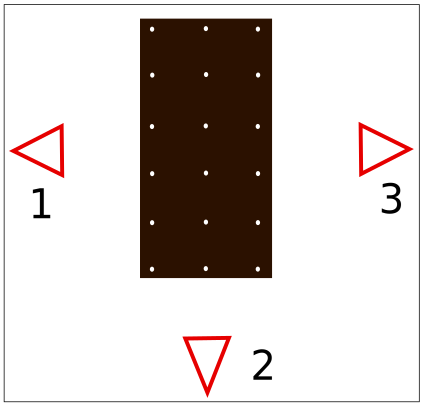
\includegraphics[scale=0.5]{img/calibracion/lab_real.pdf}
%\vspace{-0.3cm}
%\caption{Laboratorio del Hospital de Clínicas.}
%\label{fig: lab_real}
%\end{figure}


%La metodología utilizada consiste en el uso de tres cámaras de video convencionales de 25 fps y resolución  720 x 576 píxeles. Dichas cámaras se disponen como se muestra en la Figura \ref{fig: lab_real}, alrededor de una alfombra o cinta sobre la que se le pide al paciente que camine.\\



%La persona que se desea evaluar debe tener colocados marcadores, fundamentalmente en las articulaciones del cuerpo, y debe desplazarse sobre la alfombra dispuesta para esto. En la Figura \ref{fig: persona con marcadores}, se observa a un individuo caminando con los marcadores colocados.

%\vspace{-0.2cm}
%\begin{figure}[ht!]		
        %\subfloat[Persona con marcadores]{\includegraphics[scale=0.28]{img/calibracion/captura_real.png}\label{fig: persona con marcadores}}
%        \hspace{0.1cm}
        %\subfloat[Objeto de calibración]{\includegraphics[trim = 20mm 0mm 40mm 0mm, clip, scale=0.28]{img/calibracion/calibrador.png}\label{fig: calibrador}}
%  \caption{Captura de secuencia real}
      \label{fig: captura real}
%\end{figure}

%Antes de la captura del movimiento se emite una señal acústica con la cual se sincronizan las tres vistas una vez obtenidos los videos. El software con el cual este grupo de médicos ha analizado el movimiento es el \textit{Dvideow}.            
 %%%%%%%%%%%%%%%%%%(REFERENCIAR)%%%%%%%%%%%%%%%%%%%%%%%%%%%%%%. 
% Dicho software realiza la detección, seguimiento y reconstrucción de los marcadores. Por otro lado, no se ha podido tener acceso a este software por lo cual tampoco se pudo evaluar su desempeño y compararlo con el desarrollado en este proyecto.\\

%El método que utilizaron para calibrar las cámaras requiere de un objeto de calibración como el que se muestra en la Figura \ref{fig: calibrador}, al que se le llama \textit{fantoma}. Este objeto se compone de marcadores colocados sobre una estructura cuyas dimensiones son conocidas. Dicho objeto se lo coloca en posiciones determinadas que se encuentran marcadas sobre la alfombra, ver Figura \ref{fig: calibrador}. De esta manera se obtiene un mayor número de puntos ubicados en el volumen de trabajo.\\


%Los videos proporcionados por los especialistas del Hospital de Clínicas incluyen tanto las secuencias de marcha de diferentes individuos como el proceso con el que se calibran las cámaras del laboratorio. A partir de dichos videos se desarrolló un algoritmo tal que permite extraer las matrices de proyección de cada una de las cámaras. Tomando un cuadro del video en el que se encuentre el \textit{fantoma} en una de las posiciones, el algoritmo implementado requiere que cada marcador del \textit{fantoma}, en cada una de las vistas, sea seleccionado manualmente, y en un orden tal que permita establecerse una correspondencia entre las proyecciones de un mismo marcador en las tres vistas. En la Figura \ref{fig: vistas_calibrador} se muestra a uno de los marcadores seleccionado en cada una de las vistas.
%\vspace{-0.53cm}
%\begin{figure}[ht!]
%        \hspace{-1cm}
        %\subfloat[Vista cámara 1]{\includegraphics[trim = 59mm 0mm 41mm 0mm, clip,scale=0.45]{img/calibracion/calibrador_cam1.png}}
%                \hspace{1mm}
       % \subfloat[Vista cámara 2]{\includegraphics[trim = 50mm 0mm 50mm 0mm, clip,scale=0.45]{img/calibracion/calibrador_cam2.png}}     	
%  \hspace{1mm}
        %\subfloat[Vista cámara 3]{\includegraphics[trim = 32mm 0mm 68mm 0mm, clip,scale=0.45]{img/calibracion/calibrador_cam3.png}}
      
%      \caption{Uno de los marcadores de calibrador seleccionado en cada una de las cámaras}
%      \label{fig: vistas_calibrador}      
%\end{figure}


%Por otra parte la posición de los marcadores en el espacio 3D es conocida ya que se saben las medidas del \textit{fantoma}, ver Figura \ref{fig: medidas_calibrador}. Dichas posiciones pueden ser referidas un punto que puede elegirse arbitrariamente, así como los ejes de coordenadas $(x,y,z)$.

%\vspace{-0.53cm}
%\begin{figure}[ht!]
%        \centering
     %{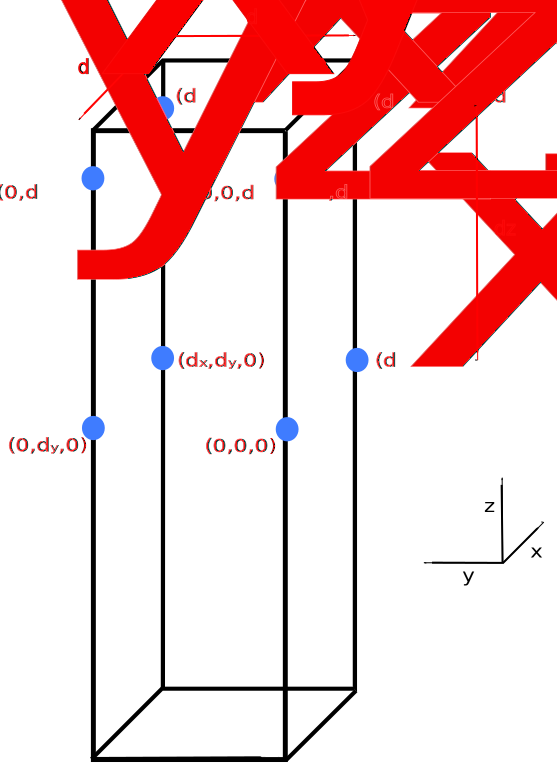
\includegraphics[scale=0.38]{img/calibracion/medidas_calibrador.pdf}}    
%     \caption{Coordenadas de los marcadores del \textit{fantoma}}
%      \label{fig: medidas_calibrador}     
%\end{figure}

%  De esta forma se tiene asociadas las coordenadas 3D de los marcadores en el espacio con sus correspondientes coordenadas 2D en píxeles en cada una de las cámaras, $\mathbf{X_i} \leftrightarrow  \mathbf{x_i}$. Si se tiene una cantidad suficiente de puntos, entonces las matrices de proyección $P$ pueden ser estimadas tal que $\mathbf{x_i}=P\mathbf{X_i}$. Para esto se utiliza el algoritmo \textit{Direct Linear Transformation (DLT)}.\\
   
% Según lo demostrado en \cite{hartley}, para cada asociación de puntos $\mathbf{X_i} \leftrightarrow \mathbf{x_i}$ se cumple que :
   
%   \[
%   \begin{pmatrix}
%   0^T & -w_iX_i^T & y_iX_i^T \\
%   w_iX_i^T & 0^T & -x_iX_i^T
%   \end{pmatrix}
%   \begin{pmatrix}
%    P^1 \\
%    P^2 \\
%    P^3
%   \end{pmatrix}
%   = 0   
%      \]
   
   
% \hspace{-0.6cm}siendo $P^{iT}$ las columnas $i$-ésimas de $P$ y $\mathbf{x_i}$ de coordenadas homogéneas $(x_i,y_i,w_i)$. Dicha matriz se obtiene resolviendo un conjunto de ecuaciones del tipo $Ap=0$.  Dado que por cada punto se tiene dos ecuaciones y que la matriz $P$ tiene doce entradas y once grados de libertad, ignorando el factor de escala, resulta que son necesarios conocer al menos seis correspondencias $X_i \leftrightarrow x_i$.\\
 
%Para anular los efectos de la selección arbitraria del origen y la escala del sistema de coordenadas se aplica una normalización tanto a los puntos imagen 2D como a los 3D, logrando de esta manera mejorar los resultados finales. Para los puntos 2D de cada vista se traslada el origen de coordenadas de dicha vista al centroide de los puntos y se aplica un escalado tal que la distancia promedio de los puntos al origen sea $\sqrt{2}$. Para los puntos 3D el mismo procedimiento excepto que el escalado que se aplica es tal que la distancia promedio al origen es $\sqrt{3}$. De esta manera se tiene dos matrices que realizan esta transformación, la matriz $T_{3D}$ tal que $\tilde{X_i} = T_{3D}^{}X_i$ para los puntos en el espacio, siendo $\tilde{X_i}$ los puntos normalizados. Análogamente para los 2D imagen se tiene la matriz $T_{2D}^{}$ tal que $\tilde{x_i} = T_{2D}^{}x_i$. \\
 
% Dado que las coordenadas de los puntos 2D están afectadas por el ruido y que se tienen más de seis correspondencias $X_i \leftrightarrow x_i$, no existe una solución exacta a las ecuaciones $Ap=0$. Por lo tanto la solución se obtiene minimizando un error, en este caso se busca $p$ tal que minimice $||Ap||$. Para esto se utiliza la descomposición en valores singulares (SVD), donde se obtiene del vector singular asociado al menor valor singular. De esta manera se obtiene la matriz de proyección $\tilde{P}$. Por último debe descomponerse la normalización, por lo tanto la matriz de proyección $P$ queda $P = T_{2D}^{-1} \tilde{P} T_{3D}^{}$.
 
%\subsection{Calibración simulada en \emph{Blender}}
 
 Con el objetivo de establecer una metodología de calibración que fuera válida para la configuración de cámaras con las que se diseñó el entorno virtual descrito en la sección \ref{section_base_de_datos}, se probaron distintas implementaciones existentes. Para esto se evaluaron dos toolbox elaborados en \emph{Matlab}. La metodología de calibración fue simulada en \emph{Blender} mediante \textit{scripts} \emph{Python} y las imágenes obtenidas como resultado se procesaron con dichos toolbox. La descripción de la metodología y las simulaciones se detalla en \cite{proyecto_biomecanica}.\
 
 Uno de los toolbox utilizados es el \textit{Automatic Multi-Camera Calibration Toolbox (amcctoolbox)} \cite{amcctoolbox}, el cual utiliza como objeto de calibración un damero. Este método, aunque sus resultados tienen buena precision \cite{zhang_libro}, puede no ser suficientemente flexible para un sistema de muchas cámaras ya que, entre otras cosas, es necesaria la intervención manual en algunos casos.\
 
El otro toolbox utilizado es el \textit{Multi-Camera Self-Calibration Toolbox} \cite{toolbox_led}. Este método consiste en capturar el movimiento de una fuente puntual de luz que recorra el volumen de trabajo. Para cada cuadro se tiene un punto 3D en el espacio en una posición distinta y en cada una de las cámaras su correspondiente proyección.
 El error de re-proyección promedio obtenido es menor a 0.13 píxeles para todas las cámaras. Este método plantea una forma simple de calibrar un conjunto de muchas cámaras adecuado para el sistema de 17 cámaras del laboratorio virtual desarrollado en \emph{Blender}.

 
 
%\subsubsection{Automatic Multi-Camera Calibration Toolbox (amcctoolbox) }\cite{amcctoolbox}  


%Esta herramienta automatiza ciertas funciones del toolbox \textit{Camera Calibration Toolbox}, reduciendo la intervención del usuario. Utiliza como objeto de calibración un damero.

%Para la calibración de conjuntos de varias cámaras, el damero debe ser colocado en múltiples ubicaciones y orientaciones cubriendo el mayor volumen de trabajo tal que, en cada una de estas posiciones, el damero pueda ser visto por más de una cámara simultáneamente.

%La calibración del entorno virtual se realiza simulando un damero real. Para cada par de cámaras adyacentes se coloca el damero en algún punto dentro del volumen de trabajo, con una orientación tal que la figura plana del damero sea visible en ambas cámaras. Luego, a partir de dicha posición, se toman capturas del damero cambiando ligeramente la ubicación y orientación del mismo. Para cada par de cámaras adyacentes se consideran entre 15 y 20 posiciones distintas del damero.

%Una vez realizadas las capturas se procesan  las imágenes mediante el toolbox, obteniéndose los parámetros intrínsecos de cada una de las cámaras y la posición relativa de cada uno de los pares de cámaras adyacentes y por lo tanto las posición relativa de todas las cámaras.


%Este método aunque sus resultados tiene buena precision \cite{zhang_libro}, puede no ser suficientemente flexible para un sistema de muchas cámaras, ya que, entre otras cosas, puede ser necesaria la intervención manual en algunos casos.



%\subsubsection{ Multi-Camera Self-Calibration Toolbox } \cite{toolbox_led}
 
 %El procedimiento utilizado en este toolbox consiste en capturar el movimiento de una fuente puntual de luz que recorra el volumen de trabajo. Por lo tanto para cada cuadro se tiene un punto 3D en el espacio en una posición distinta y en cada una de las cámaras su correspondiente proyección si dicho punto es visible desde la cámara. Para esto debe existir un contraste suficiente de la fuente puntual de luz respecto al laboratorio. La fuente de luz puede ser por ejemplo, una lámpara led.
 
%La simulación de este procedimiento se logra creando un punto 3D que toma para cada cuadro, distintas posiciones en forma aleatoria dentro del volumen de trabajo. Para cada cuadro se \textit{renderiza} su posición en las 17 cámaras. En este caso se han tomado 500 posiciones distintas.

% El error de re-proyección promedio obtenido es menor a 0.13 píxeles para todas las cámaras. Este método plantea una forma simple de calibrar un conjunto de muchas cámaras adecuado para el sistema de 17 cámaras del laboratorio virtual desarrollado en \emph{Blender}.

%En la Figura \ref{fig: error reproyeccion} se muestra en azul el promedio y en rojo la desviación estándar del error de re-proyección obtenido para cada una de las cámaras. Sea $X$ un punto 3D en el espacio cuya posición es a priori desconocida y $x$ su correspondiente proyección en un cámara. A partir del resultado de la calibración se obtiene la matriz de proyección $P$ de dicha cámara. A su vez, es posible obtener la estimación del  punto $X$, siendo $ \hat{X}$ dicha estimación. La proyección de $\hat{X}$ sobre la cámara es $\hat{x} = P \hat{X}$. El error de re-proyección de $\hat{X}$ se define como la distancia euclídea $d(x,\hat{x})$ entre los vectores $x$ y $\hat{x}$.\\

%\begin{figure}[ht!]
%\begin{center}
%\includegraphics[scale=0.5]{img/calibracion/reprerrors.pdf}
%\end{center}
%\caption{Promedio y desviación estándar del error de re-proyección en todas las cámaras }
%\label{fig: error reproyeccion}
%\end{figure}
  
  
%  Como se observa de la Figura se obtienen errores menores a 0.13 píxeles para todas las cámaras.
  
%\subsubsection{Ajuste del sistema de coordenadas.}

%De los dos toolbox vistos anteriormente se obtuvieron los parámetros intrínsecos y extrínsecos de las cámaras. En el \textit{Multi-Camera Self-Calibration Toolbox} las parámetros extrínsecos de las cámaras son referidos a un sistema de coordenadas desconocido que se establece en el proceso de calibración del toolbox. El origen de coordenadas de ese sistema se ubica en el centroide de todas las posiciones capturadas de la fuente de luz. En el \textit{amcctoolbox} por otra parte, los parámetros extrínsecos de las cámaras son referidos al sistema de coordenadas de la cámara que se definió como el origen del sistema de coordenadas.\\

 %En algunos casos puede desearse que el sistema de coordenadas del espacio 3D sea definido por el usuario. En nuestro caso para poder comparar el resultado de la calibración con el ground truth, el sistema de coordenadas al que están referidos los parámetros de la calibración, debe coincidir con el sistema de coordenadas  definido en el entorno \emph{Blender}.\\

%Una opción para realizar esto, es colocar en el espacio marcadores en posiciones conocidas y capturar imágenes de dichos marcadores en cada cámara. Se asume que de la calibración se obtuvieron las matrices de proyección para cada una de las cámaras referidas a un sistema de coordenadas del espacio, \textit{a priori}, desconocido. Sea entonces, $S_1$ dicho sistema de coordenadas, y $P_i|_{S_1}$ las matrices de proyección referidas a este sistema, siendo $i$ la $i$-ésima cámara. Sea $S_2$ el sistema de coordenadas que se desea establecer como el nuevo sistema de referencia del espacio 3D, y $P_i|_{S_2}$ las matrices de proyección referidas a este sistema, que se deben encontrar.\\

%Si se colocan marcadores en determinadas posiciones del espacio, entonces son conocidas sus coordenadas respecto al sistema $S_2$. Sean $X_j|_{S_2}$ sus coordenadas 3D en el sistema $S_2$, siendo $j$ el $j$-ésimo marcador. Dichos puntos se proyectan en las cámaras en los puntos de coordenadas 2D $x_j^i$. Con dichos puntos y las correspondientes matrices de proyección $P_i|_{S_1}$ es posible conocer las coordenadas de los puntos $X_j$ respecto al sistema $S_1$, esto es, $X_j|_{S_1}$. Con lo cual se tienen las coordenadas de los $j$ marcadores en ambos sistemas de coordenadas. De esta manera es posible inferir la transformación $Tr$ tal que $Tr(X_j|_{S_1}) = X_j|_{S_2}$. Si se aplica el cambio de base a las matrices de proyección se obtiene $Tr(P_i|_{S_2}) = P_i|_{S_1} $. Dicha transformación es una composición de una traslación y una rotación.


%\subsection{Conclusiones}

%En el presente capítulo se han tratado varios métodos de calibración y se ha expuesto porqué dicho proceso es necesario para conocer los parámetros de las cámaras en sistemas de captura. Se ha visto además que de la calibración se obtienen ciertos parámetros que son intrínsecos y otros extrínsecos a las cámaras, basados en el modelo \textit{pinhole} de cámara. Por otra parte se describe cómo obtener los parámetros de calibración a partir de la información proporcionada por el entorno \emph{Blender}, esto último permite conocer el \textit{ground truth} de la calibración para un conjunto de cámaras así como el \textit{ground truth} de la detección de marcadores en las imágenes 2D.\\

%Se implementó un algoritmo que realiza la calibración de cámaras, para la metodología particular utilizada en la captura de movimiento realizada a pacientes en el Hospital de Clínicas. Dicha metodología plantea la utilización de una estructura tridimensional con marcadores ubicados convenientemente. Una característica de este método es que permite abarcar todo el volumen de trabajo. Asimismo el uso de objetos 3D para la calibración ofrece mayor precisión \cite{zhang_libro}. Sin embargo, tiene como desventaja que requiere la intervención del usuario en el proceso de calibración, con lo cual resulta en un metodología poco adecuada para calibrar un sistema de muchas cámaras.\\



%el metodo para el caso real permite abarcar todo el volumen de trabajo, tiene mayor precision pero requiere la interviencion del usuario  por lo que no es adecuado para calibrar un conjunto de muchas camaras.




%Por otra parte se han utilizado dos toolbox elaborados en \emph{Matlab}, para calibrar las cámaras del laboratorio virtual implementado en \emph{Blender}. Para esto se ha simulado en el mismo entorno \emph{Blender} una calibración real utilizando estos toolbox.\\


%El \textit{amcctoolbox}, plantea un método muy utilizado para la calibración de cámaras a través de objetos planos, en nuestro caso un damero, cuyos resultados poseen buena precisión \cite{zhang_libro}. Sin embargo presenta la desventaja de que los parámetros extrínsecos de las cámaras se vinculan en relación a sus adyacentes, por lo que debe definirse a una de las cámaras como el origen del sistema de coordenadas del espacio, respecto a la cual se halla la posición del resto de las cámaras. Por lo tanto el error se acumula incrementándose en aquellas cámaras que están más alejadas de aquella que se define como el origen del sistema. Este toolbox por otra parte, requiere para la calibración de un par cámaras, establecer en forma automática una correspondencia entre la imagen del damero detectado en la cámara izquierda con la imagen capturada por la cámara derecha. Esto en algunos casos no se logra y la correspondencia entre dichas imágenes debe realizarse en forma manual. \\





%Debe considerarse para trabajos futuros, además de los aspectos cualitativos expuestos,  una evaluación de performance de los métodos considerados, teniendo en cuenta las diferencias implicadas en la calibración de un sistema de pocas o muchas cámaras.\\
\clearpage
\subsection{Reconstruction}
Segmentation output has, for each camera and for each frame of a sequence, a set of coordinates $(x, y)$ that locate the position in the image of detected markers.
The reconstruction process is to obtain the position of the markers in space, from 2D markers position in at least two retinas.

The reconstruction process presented was inspired by Herda's work and consists of three basic steps:
\vspace{-0.2cm}
\begin{enumerate}
\item Find the correspondence between points in different retinas.
\item Select best match.
\item Reconstruct and check rest of the retinas.
\end{enumerate}
\vspace{-0.8cm}
\subsubsection{Algorithm}
The implemented algorithm receives as input 2D points of detected markers and returns as output reconstructed 3D points.
Figure \ref{fig: diagrama algoritmo} is a diagram of the algorithm presented.
%\vspace{-0.2cm}
\begin{figure}
    \begin{center}
        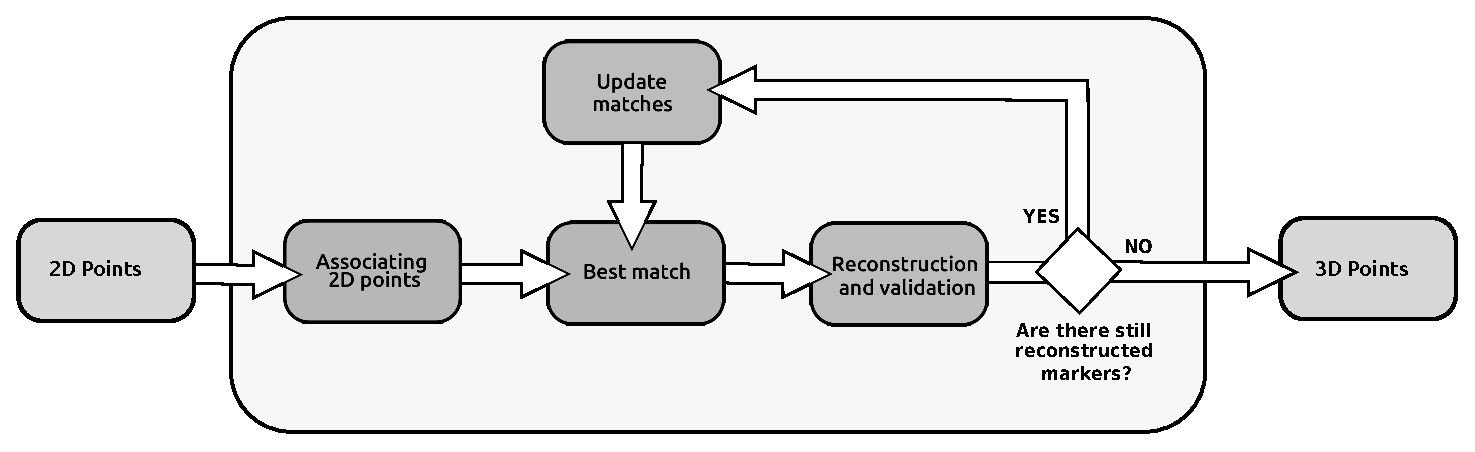
\includegraphics[scale=0.45]{./imagenes/Reconstruccion/bloques_reconstruccion}
        \caption{Block diagram of reconstruction algorithm.}
        \label{fig: diagrama algoritmo}
    \end{center}
\end{figure}
%\vspace{-0.6cm}

\textit{Associating 2D points.}\label{seccion_asociar2D_uno}
%
This block receives as input the coordinates of detected points and projection matrices of the cameras, returning to each point a list sorted by relevance of the existing partnerships with points on other cameras. \\ 
\textit{\hspace*{0.5cm}Best match.}\label{MejorAsociacion}
%
From the list of associations between pairs of cameras it is necessary to choose one that possesses more probability to form the pair corresponding to the projection of a 3D marker views on such images.
%
From each pair of cameras is taken the association which maintains the shorter distance and contains valid points, discarding the rest. 
\vspace{-0.65cm}
\begin{figure}
    \begin{center}
       \includegraphics[scale=1.0]{./imagenes/Reconstruccion/Algoritmo_reconstruccion}       
    \end{center}
\end{figure}
\vspace{-1.0cm}

To choice the pairs of cameras were considered two cases.
The first one evaluates each camera with all remaining and the second one considers the arrangement of cameras in space and match the adjacent cameras consecutively.

\textit{3D reconstruction and Validation.}\label{seccion_reconstruccion3D_validacion}
Couple of points $x_i x_j$ of cameras $i$ and $j$ respectively, reconstruct a valid point 3D $X_{ij}$ if there is at least one $x_k$ in camera $k\not= i, \,j$ such that $X_{ik} \in $ sphere$(X_{ij}, \delta)$, to certain threshold $\delta$.

\textit{Update matches}\label{actualizar_asociaciones}
The couple who reconstructs $X_{ij}$ as well as $x_k$ points who validate this reconstruction are removed. 
Iteration continue repeating the process with next pairs of best associated cameras.
Finally iterative process stops when the number of reconstructed markers equals number of markers that the person has, equal to maximum number of reconstructions indicated, or not valid 2D points such that a partnership between different points of view can be established.
\clearpage
\subsection{Seguimiento}

The tracking of marker trajectories is performed by a sliding window of three or four frames linking the reconstructed points under the assumption that displacement of a marker from one frame into the next is minimal. This methodology was used by Herda \textit{et al.} \cite{herda} based on the work of Malik \textit{et al.} \cite{griegos}.

\hspace*{0.5cm} \textit{Algorithm}. Being known the trajectory of a marker until frame [f]  it's wanted to find the next position on frame [f+1] which is predicted by the displacement from [f-1] to [f]. A search neighbourhood is defined centered on the predicted point in which is expected to find the best reconstructed marker that continues the trajectory.

If within the search neighbourhood there is more than one posible candidate, for each of them is defined a second prediction on frame [f+2] such that the acceleration from [f-1], [f] and the predicted point in [f+1] is the same as the acceleration of [f+1] and the predicted point in [f+2]. Then is selected the trajectory whith the least variation of acceleration. If there is not any marker within the search neighbourhood  its radius is expanded up to a limit. If a trajectory could not be linked in a frame, the movement is prolonged into the next frames to find reconstructed markers near the predicted ones so the markers between those frames can be extrapolated. In addition, thresholds are implemented to define limits on the acceleration to detect discontinuities on the tracking. Figure \ref{restricciones_tracking} shows the motion capture of a walk standing out the trajectories of the leg markers.

\begin{figure}[ht!]
 \begin{center}
%  \subfloat[Trayectorias de marcadores de pierna]
  {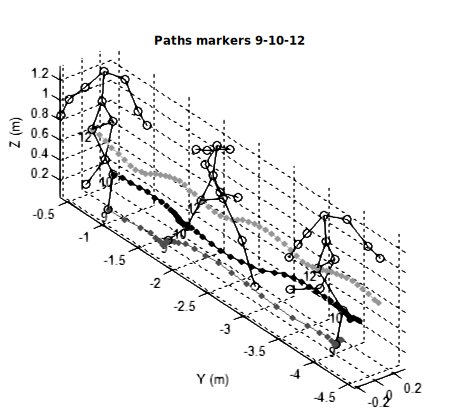
\includegraphics[scale=0.4]{imagenes/Seguimiento/050_Salida_Tracking_13_14_10} %\label{trayectorias_marcadores_piernas}
   }	
 % \subfloat[Distancia y Angulo entre marcadores de la pierna.]
 {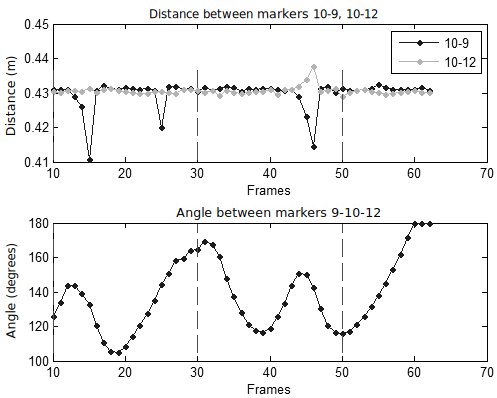
\includegraphics[scale=0.4]{imagenes/Seguimiento/051_Salida_Angulo_Distancia_13_14_10}\label{distancia_angulo_marcadores_piernas}}
  \end{center}
\caption{\textit{Left}: leg markers trajectories. \textit{Right}: distance and angle between two leg markers.}
\label{restricciones_tracking}
\end{figure}


Another tracking algorithms could be used like Kalman \cite{kalman} which requires the inicialization of models. There are also algorithms based on the constraint that some markers keep a constant distance between them.

%
%
%\subsection{Seguimiento}
%
%El seguimiento de trayectorias se realiza sobre una ventana deslizante de tres a cuatro cuadros enlazando los puntos reconstruidos de manera de mantener un movimiento lo mas suave posible. 
%Esta metodología fue utilizada por Herda \cite{herda} en su trabajo basándose en los estudios de Malik, Drako, Papantoniou \cite{griegos} .
%
%
%\hspace*{0.5cm} \textit{Algoritmo.} Sea la trayectoria de un marcador enlazada hasta el instante [f] sobre la cual desea buscarse su próximo punto en [f+1], el movimiento entre [f-1] y [f] es prolongado para establecer un centro de búsqueda y encontrar el punto reconstruido que mejor continúa la trayectoria como se muestra en la Figura \ref{herda_00} .
%
%%\vspace{-0.7cm}
%\begin{figure}[ht!]
%\begin{center}
%\includegraphics[scale=0.4]{imagenes/Seguimiento/tracking-eps-converted-to.pdf}
%\end{center}
%\caption{Seguimiento en cuatro cuadros, siendo [f] el cuadro actual que queremos seguir en [f+1]. ( Fuente  Human movement
%science 20(3), 313–341 \cite{herda} ) .}
%\label{herda_00}
%\end{figure}
%%\vspace{-0.3cm}
%Se presentan tres posibles casos al buscar puntos reconstruidos:
%
%\begin{itemize}
%
%\item Si solo se encuentra un punto reconstruido se agrega a la trayectoria para el cuadro [f+1], buscando el mas cercano a la estimación calculada como aquella que mejor se aproxima a una trayectoria de tres puntos con aceleración mínima
%
%\item En el caso de encontrar mas de un punto cada posible candidato es evaluado para realizar una segunda estimación hacia [f+2] de forma que la aceleración entre [f-1], [f] y el candidato en [f+1] sea la misma que entre [f], el candidato en [f+1] y la estimación en [f+2]. Luego de todos los posible caminos en cuatro cuadros, se elige el de menor variación de aceleración.
%
%\item Si no se encuentra ningún punto, se procede a aumentar de forma limitada el radio de búsqueda en [f+1] de forma excepcional. Esto se hace para continuar trayectorias que entran en estado de reposo y el último movimiento conocido es nulo o muy pequeño.
%
%\end{itemize}
%
%Si una trayectoria queda trunca durante el enlazado, se intenta recuperar prolongando el movimiento en próximas cuadros para encontrar puntos reconstruidos cercanos a las estimaciones y extrapolar los puntos intermedios. Por otro lado, se implementan umbrales para definir límites sobre la aceleración de los enlaces obtenidos y detectar discontinuidades durante el seguimiento.
%
%Estas medidas permiten detectar trayectorias individuales sobre los puntos reconstruidos, detectar de forma simple posibles discontinuidades, y estimar reemplazos en casos de pérdidas. La captura en la Figura \ref{restricciones_tracking} corresponde a la marcha y se resaltan las trayectorias individuales de puntos de la pierna así como un esqueleto simple generado para visualizar la evolución entre marcadores.\\
%%\vspace{-0.25cm}
%\begin{figure}[ht!]
% \begin{center}
%%  \subfloat[Trayectorias de marcadores de pierna]
%  {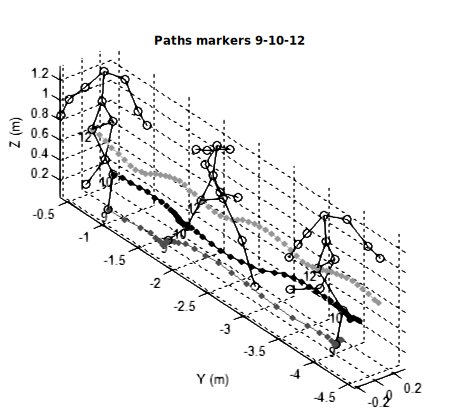
\includegraphics[scale=0.4]{imagenes/Seguimiento/050_Salida_Tracking_13_14_10} %\label{trayectorias_marcadores_piernas}
%   }	
% % \subfloat[Distancia y Angulo entre marcadores de la pierna.]
% {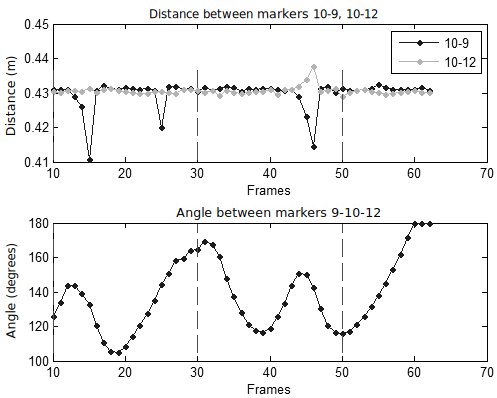
\includegraphics[scale=0.4]{imagenes/Seguimiento/051_Salida_Angulo_Distancia_13_14_10}\label{distancia_angulo_marcadores_piernas}}
%  \end{center}
%\caption{Posibles restricciones en ángulo y distancia, para el caso de la pierna en marcha. Izquierda: trayectorias de marcadores de pierna. Derecha: distancia y ángulo entre marcadores de la pierna.}
%\label{restricciones_tracking}
%\end{figure}
%%\vspace{-0.5cm}
%El conjunto de puntos reconstruidos puede ser sometido a otros algoritmos de seguimiento como Kalman \cite{kalman} requiriendo la inicialización de modelos, o algoritmos basados en restricciones más fuertes que utilicen las distancias relativamente constantes entre marcadores de los miembros y ángulos continuos entre articulaciones, requiriendo un mayor estudio de las características del sujeto y movimiento a capturar. %La Figura \ref{restricciones_tracking} muestra posibles restricciones en la marcha sobre los huesos de la pierna.
%

\clearpage
\section{Evaluación}

\subsection{Medida de Error}

Tanto para el caso de la segmentación de los vídeos como la reconstrucción de los marcadores, se tiene los verdaderos marcadores generados en la secuencia, por lo que es necesario establecer una medida de error sobre la salida de los algoritmos. Se eligió aplicar una metodología basada en la distancia euclidiana promedio, entre los marcadores de ambos conjuntos \cite{humaneva} . 

Asumiendo que los conjuntos de datos de salida de algoritmos y ground truth, tienen sus cuadros sincronizados temporalmente, en un cuadro [f] dado se tienen $M$ marcadores en un conjunto $ \boldsymbol{x},\quad\{m_{i}(x)\},i=1,\ldots,M $ , donde $ m_{i}(x)\in{\mathbf{R}^{3}} $ ( o $ \mathbf{R}^{2} $ para el caso de las vistas de cámaras individuales), y $ \boldsymbol{\tilde{x}} $ es el conjunto ground truth con la misma cantidad $M$ de marcadores alineados con $\boldsymbol{x}$ (el $i$-esimo marcador de $\boldsymbol{x}$ se corresponde con el  $i$-esimo marcador de $\boldsymbol{\tilde{x}}$), se calcula la distancia como

\begin{equation}
D(\boldsymbol{x_{f}},\boldsymbol{\tilde{x_{f}}})=\frac{1}{M}\sum_{i=1}^{M} \|m_{i}^{[f]}(\boldsymbol{x})-m_{i}^{[f]}(\boldsymbol{\tilde{x}})\|
\label{error_vs_ground_basica}
\end{equation}

Sin embargo, el calculo debe ser modificado para contemplar para el caso en que la cantidad de marcadores a la salida del procesamiento es menor a $M$, se define un conjunto binario en cada frame $\Delta=\{\delta_1,\delta_2,\ldots,\delta_M\}$, donde $\delta_i$ indica con 1 si el $i$-esimo marcador de $\boldsymbol{\tilde{x}}$ fue detectado, 0 en caso contrario. La ecuación \ref{error_vs_ground_basica} queda entonces

\begin{equation}
D(\boldsymbol{x_{f}},\boldsymbol{\tilde{x_{f}}},\Delta_{f})=\frac{1}{\sum_{j=1}^{M} \delta_j} \sum_{i=1}^{M} \delta_i.\|m_{i}^{[f]}(\boldsymbol{x})-m_{i}^{[f]}(\boldsymbol{\tilde{x}})\|
\label{error_vs_ground_deteccion}
\end{equation}

En una secuencia con $F$ frames, la performance promedio es calculada como el promedio de los errores en cada frame,

\begin{equation}
\mu_{secuencia} = \frac{1}{F}\sum_{f=1}^{F} D(\boldsymbol{x_{f}},\boldsymbol{\tilde{x_{f}}},\Delta_{f})
\label{performance_secuencia}
\end{equation}

Para poder trabajar con los datos a la salida de la segmentación y reconstrucción de las secuencias, es necesario obtener datos adicionales y entonces aplicar la ecuación \ref{performance_secuencia}. Específicamente, las parejas entre marcadores obtenidos y aquellos en el ground truth , que permite alinear y comparar los marcadores, y definir cuales fueron detectados.

El emparejamiento es realizado frame a frame, calculando en una matriz la distancia euclidiana entre todos los pares $\{i,j\}$, donde $i=1,\ldots,M_{x}$ es un marcador del conjunto $\boldsymbol{x}$ obtenido mediante algoritmo en un frame [f], y $j=1,\ldots,M_{\tilde{x}}$ es un marcador del conjunto $\boldsymbol{\tilde{x}}$ de ground truth,

\begin{equation}
d_{i,j}^{[f]} = \{\|m_{i}^{[f]}(\boldsymbol{x})-|m_{j}^{[f]}(\boldsymbol{\tilde{x}})\|\}
\label{distancia_algoritmo_ground}
\end{equation}

Una vez calculadas todas las distancias para un frame, se buscan aquellas parejas que presenta la menor distancia, relevando la pareja $(i,j)$  para la cual se verifica. Una vez obtenida esta distancia, los marcadores $(i,j)$ quedan descartados de la matriz, volviendo a buscar la siguiente pareja con distancia mínima, hasta que ya no queden elementos para emparejar (lo cual sucede en caso que se generen menos marcadores que en el ground truth como puede suceder en segmentación, o si todos los marcadores de ground truth ya fueron emparejados y sobran marcadores, como sucede en reconstrucción). Trabajar con las parejas en todos los grames de la secuencia, es análogo a trabajar con la ecuación (\ref{error_vs_ground_deteccion}) .

\subsection{Performance}

\subsubsection{Capturas Sintéticas}

Resultados múltiples secuencias

\begin{table}[h]
\begin{tabular}{cccc|c|c|c|c|c|c|ll}
\cline{5-10}
                              &                                 &                             &         & SEGM.                                                   & SEGM.                                               & RECONS.                                                 & RECONS.                                             & TRACK.                                                  & TRACK.                                              &  &  \\ \cline{1-10}
\multicolumn{1}{|c|}{captura} & \multicolumn{1}{c|}{markers} & \multicolumn{1}{c|}{frames} & n.cams & \begin{tabular}[c]{@{}c@{}}Promedio\\ (px)\end{tabular} & \begin{tabular}[c]{@{}c@{}}99\%\\ (px)\end{tabular} & \begin{tabular}[c]{@{}c@{}}Promedio\\ (cm)\end{tabular} & \begin{tabular}[c]{@{}c@{}}99\%\\ (cm)\end{tabular} & \begin{tabular}[c]{@{}c@{}}Promedio\\ (cm)\end{tabular} & \begin{tabular}[c]{@{}c@{}}99\%\\ (cm)\end{tabular} &  &  \\ \cline{1-10}
\multicolumn{1}{|c|}{8,03,1}  & \multicolumn{1}{c|}{14}         & \multicolumn{1}{c|}{89}     & 17      & 1,1063                                                  & 3,6783                                              & 0,40778                                                 & 2,6384                                              & 0,4318                                                  & 2,9039                                              &  &  \\ \cline{1-10}
\multicolumn{1}{|c|}{8,07,1}  & \multicolumn{1}{c|}{14}         & \multicolumn{1}{c|}{62}     & 17      & 1,0871                                                  & 3,1172                                              & 0,34382                                                 & 1,806                                               & 0,34451                                                 & 1,806                                               &  &  \\ \cline{1-10}
\multicolumn{1}{|c|}{8,07,2}  & \multicolumn{1}{c|}{14}         & \multicolumn{1}{c|}{123}    & 17      & 1,0912                                                  & 3,3097                                              & 0,38736                                                 & 1,2681
& 0,36381                                                 & 1,2681                                              &  &  \\ \cline{1-10}
\multicolumn{1}{|c|}{8,11}    & \multicolumn{1}{c|}{13}         & \multicolumn{1}{c|}{94}     & 17      & 1,074                                                   & 2,9042                                              & 0,38836                                                 & 2,8705                                              & 0,38836                                                 & 2,8705                                              &  &  \\ \cline{1-10}
\multicolumn{1}{|c|}{9,07,1}  & \multicolumn{1}{c|}{14}         & \multicolumn{1}{c|}{29}     & 17      & 1,1285                                                  & 3,3211                                              & 0,28016                                                 & 2,0401                                              & 0,28016                                                 & 2,0401                                              &  &  \\ \cline{1-10}
\multicolumn{1}{|c|}{9,07,2}  & \multicolumn{1}{c|}{14}         & \multicolumn{1}{c|}{57}     & 17      & 1,1404                                                  & 3,4476                                              & 0,34517                                                 & 1,9902                                              & 0,34517                                                 & 1,9902                                              &  &  \\ \cline{1-10}
\multicolumn{1}{|c|}{9,12,1}  & \multicolumn{1}{c|}{13}         & \multicolumn{1}{c|}{300}    & 15      & 1,0443                                                  & 2,118                                               & 0,39731                                                 & 1,4952                                              & 0,39741                                                 & 1,4952                                              &  &  \\ \cline{1-10}
\end{tabular}
\caption{Resultados de los bloques, para distintas capturas sintéticas}
\label{resultados_distintas_capturas}
\end{table}

\subsubsection{Ruido En Segmentación}

Resultado Reconstrucción (cm) ,ingresando Cam + ruido en pixel

\begin{table}[h]
\begin{tabular}{|c|c|c|c|c|c|}
\hline
\textbf{Caso} & \textbf{\begin{tabular}[c]{@{}c@{}}Ruido\\ (px)\end{tabular}} & \textbf{\begin{tabular}[c]{@{}c@{}}14\\ Reconstr.\end{tabular}} & \textbf{\begin{tabular}[c]{@{}c@{}}18\\ Reconstr.\end{tabular}} & \textbf{\begin{tabular}[c]{@{}c@{}}30\\ Reconstr.\end{tabular}} & \textbf{\begin{tabular}[c]{@{}c@{}}46\\ Reconstr.\end{tabular}} \\ \hline
Ground Cam    & 0                                                             & 7,84E-07                                                        & 7,84E-07                                                        & 7,84E-07                                                        & 7,84E-07                                                        \\ \hline
Segmentación  & 0                                                             & 1,5792                                                          & 0,38556                                                         & 0,38556                                                         & 0,38556                                                         \\ \hline
Ground Cam    & 0,5                                                           & 4,0817                                                          & 0,45675                                                         & 0,4453                                                          & 0,42607                                                         \\ \hline
Segmentación  & 0,5                                                           & 13,6991                                                         & 0,61128                                                         & 0,61381                                                         & 0,60517                                                         \\ \hline
Ground Cam    & 1                                                             & 16,9275                                                         & 0,82309                                                         & 0,72011                                                         & 0,73301                                                         \\ \hline
Segmentación  & 1                                                             & 11,0847                                                         & 0,8557                                                          & 0,82286                                                         & 0,83073                                                         \\ \hline
Ground Cam    & 2                                                             & 19,7131                                                         & 1,7649                                                          & 1,2152                                                          & 1,2027                                                          \\ \hline
Segmentación  & 2                                                             & 15,9698                                                         & 1,9701                                                          & 1,3021                                                          & 1,2884                                                          \\ \hline
Ground Cam    & 4                                                             & 28,6943                                                         & 6,1386                                                          & 2,1877                                                          & 2,0468                                                          \\ \hline
Segmentación  & 4                                                             & 51,4025                                                         & 5,7738                                                          & 2,1484                                                          & 2,1335                                                          \\ \hline
Ground Cam    & 8                                                             & 53,9555                                                         & 14,3684                                                         & 5,4929                                                          & 3,8377                                                          \\ \hline
Segmentación  & 8                                                             & 264,8935                                                        & 13,1539                                                         & 4,7142                                                          & 3,7993                                                          \\ \hline
\end{tabular}
\caption{Resultados de Error Promedio (cm) en reconstrucción, para distintos caso de ruido en la segmentación, tanto resultados sobre vídeos como sobre ground truth}
\end{table}

Mas ruido implica mas incertidumbre en la reconstrucción, mientras mas ruidos, mas marcadores reconstruidos se precisan en reconstrucción para compensar la precision. Para mayor cantidad de marcadores en reconstrucción, se hace inviable la identificación de marcadores en tracking ?

\subsubsection{Variación Cantidad de Cámaras}

Reconstrucción con menos cámaras

Con menos cámaras, según que movimiento se está capturando indica que marcadores se ven afectados en reconstrucción


Comportamiento caso real?



%\clearpage
%\section{Discusión y análisis de resultados}

\clearpage
\section{Conclusiones}

Se obtuvo en forma íntegra un sistema óptico de captura de movimiento basado en marcadores, que a partir de las capturas de video de una persona en un ambiente de laboratorio con las condiciones adecuadas, obtiene la posición 3D de  los marcadores presentes en el cuerpo de dicha persona, logrando representar su movimiento con una precisión del orden del centímetro.
%
%Si bien inicialmente el objetivo fue que el sistema funcionara por lo menos para el caso de uso de la marcha, se han probado otros  movimientos con resultados aceptables. La aplicación desarrollada permite a partir de múltiples capturas de vídeo de un sujeto en movimiento, detectar los marcadores en cada toma de video. Junto a la información de las cámaras, luego reconstruye la posición de los marcadores en el espacio y finalmente logra identificar cada marcador a lo largo de la secuencia temporal. Cabe destacar que el sistema implementado no es solo óptico, sino que es lo bastante general para funcionar con cualquier sistema de adquisición que genere imágenes, por ejemplo con imágenes infrarrojas provenientes de sistemas de captura modernos.

Por otro lado, la implementación separa cada etapa del proceso en módulos distintos, capaces de funcionar de manera independiente. Lo cual permite que el sistema no sea estrictamente óptico sino lo bastante general como para funcionar con cualquier sistema de adquisición que genere imágenes. %Esto además permite aumentar la reproductibilidad en el área, puse se cuenta con un sistema completo y esrtructurado donde fácilmente se pueden modificar, ingresar y probar distintas partes comparando sus desempeños.\\

Al realizar pruebas con secuencias reales  provenientes de tres cámaras en un laboratorio fuera de las hipótesis de captura, se producen problemas en las etapas de segmentación y reconstrucción. Efectuando extracción de fondo y modificaciones sobre la reconstrucción se logran mejores resultados aunque apenas aceptables. Constatando el fuerte impacto que tiene una pobre metodología de captura sobre el posterior procesamiento.

Se logra contribuir con reproductibilidad y metodología de diseño en el área a través de un sistema completo y estructurado de captura de movimiento.
%Para comparar los desempeños se definieron una serie de métricas, mediante las cuales se obtuvo una medida de performance de las etapas del sistema y del sistema completo, de forma tal de tener valores de referencia sobre los cuales comparar futuras versiones u otros sistemas.
\clearpage
\chapter{Clasificación de la bibliografía recopilada}
\label{tablabiblio}
A continuación se muestra una tabla con la clasificación de los documentos recopilados durante la etapa de investigación en este proyecto.

Los mismos están clasificados según las etapas que componen el sistema y tienen un código de color de acuerdo a la relevancia que tienen para el proyecto:
\begin{itemize}
	\item Verde: el documento contiene información de valor para el proyecto, por lo que debe tenerse en cuenta.
	\item Amarillo: la información contenida en el documento, si bien está relacionada con la categoría en la cual está ubicada, no contiene la metodología elegida para la implementación, o no aporta información de valor. 
\end{itemize}

Además, se agregan comentarios sobre el contenido de los documentos, el año en que fueron publicados, cantidad de citas en otras publicaciones, y ventajas y desventajas de la metodología aplicada.

\includepdf[pages={1}]{Resumen_bibliografia.pdf}

\clearpage
\section{Apéndice II: Interfaz gráfica (GUI)}

Se implementó una interfaz gráfica de forma tal de ejecutar el sistema implementado de forma más práctica. Tanto para el proceso de principio a fin, como para cada bloque por separado.

Esto último permite obtener los datos de salida de cada bloque sin necesidad de ejecutar el proceso entero ahorrando tiempo de procesamiento.

Como era de esperarse, la interfaz gráfica tiene, entre otras cosas, todos los parámetros que se le ingresan al proceso en cada módulo, por ejemplo: umbral fijo y filtro de área en el bloque de segmentación, marcadores totales, cámaras a utilizar para la reconstrucción, o el rango de frames donde se procesarán los marcadores.

En la figura \ref{guiVent} se observa una captura de pantalla de la interfaz implementada.

\begin{figure}[H]
\begin{center}
\includegraphics[scale=0.6]{img/gui.png}
\end{center}
\caption{Vista de la interfaz gráfica implementada.}
\label{guiVent}
\end{figure}

Cabe destacar que esta interfáz no pretende ser la interfáz final de la aplicación, sino un bosquejo, ya que el estado actual de la del sistema no permite que sea definido como ``aplicación de usuario'' sino como el estudio y la implementación de un sistema de captura de movimiento diseñado previamente.

Queda como pendiente, preferiblemente para un proyecto de ingeniería de sistemas, diseñar una interfaz de usuario completa, amigable y con mejor usabilidad para los especialistas que utilizarán el sistema.
\clearpage
\section{Apéndice III: Performance en conjuntos de 5 y 4 cámaras}


\begin{table}[h]
\centering
\begin{tabular}{c|c|c|c|c|c|}
\cline{2-6}
\textbf{} & \textbf{CONJUNTO} & \textbf{C5.1} & \textbf{C5.1} & \textbf{C5.2} & \textbf{C5.2} \\ \hline
\multicolumn{1}{|c|}{\textbf{MARKER}} & \textbf{NOMBRE} & \textbf{\begin{tabular}[c]{@{}c@{}}Promedio\\ (cm)\end{tabular}} & \textbf{\begin{tabular}[c]{@{}c@{}}99\%\\ (cm)\end{tabular}} & \textbf{\begin{tabular}[c]{@{}c@{}}Promedio\\ (cm)\end{tabular}} & \textbf{\begin{tabular}[c]{@{}c@{}}99\%\\ (cm)\end{tabular}} \\ \hline
\multicolumn{1}{|c|}{1} & LeftUpLeg & PERDIDO & PERDIDO & PERDIDO & PERDIDO \\ \hline
\multicolumn{1}{|c|}{2} & LeftLeg & 0,4295 & 2,3917 & 0,8971 & 22,988 \\ \hline
\multicolumn{1}{|c|}{3} & LeftFoot & 0,4147 & 0,7458 & 0,5518 & 8,6042 \\ \hline
\multicolumn{1}{|c|}{4} & RightUpLeg & 4,2922 & 58,0209 & PERDIDO & PERDIDO \\ \hline
\multicolumn{1}{|c|}{5} & RightLeg & 3,3777 & 61,5332 & 0,3934 & 1,5824 \\ \hline
\multicolumn{1}{|c|}{6} & RightFoot & PERDIDO & PERDIDO & 0,493 & 4,8055 \\ \hline
\multicolumn{1}{|c|}{7} & Spine & 18,9827 & 50,6854 & 16,6915 & 35,0544 \\ \hline
\multicolumn{1}{|c|}{8} & Head & 9,2659 & 22,7929 & PERDIDO & PERDIDO \\ \hline
\multicolumn{1}{|c|}{9} & LeftArm & 0,5064 & 4,9531 & 0,3648 & 0,5347 \\ \hline
\multicolumn{1}{|c|}{10} & LeftForeArm & 0,6575 & 10,2007 & 0,7586 & 13,8037 \\ \hline
\multicolumn{1}{|c|}{11} & LeftHand & 0,6831 & 13,8355 & 1,5395 & 25,0238 \\ \hline
\multicolumn{1}{|c|}{12} & RightArm & 0,7107 & 14,7915 & 0,6703 & 7,409 \\ \hline
\multicolumn{1}{|c|}{13} & RightForeArm & 2,3882 & 34,3833 & PERDIDO & PERDIDO \\ \hline
\multicolumn{1}{|c|}{14} & RightHand & 1,906 & 38,9179 & PERDIDO & PERDIDO \\ \hline
 & \textbf{Secuencia} & \textbf{3,0121} & \textbf{40,035} & \textbf{1,0513} & \textbf{20,5912} \\ \cline{2-6} 
\end{tabular}
\label{error_captura_marcha_5_camaras}
\caption{Error de Marcadores en Tracking para conjuntos de 5 cámaras en el caso de Marcha}
\end{table}

\begin{table}[h]
\centering
\begin{tabular}{c|c|c|c|c|c|}
\cline{2-6}
\textbf{} & \textbf{CONJUNTO} & \multicolumn{2}{c|}{\textbf{C4.1}} & \multicolumn{2}{c|}{\textbf{C4.2}} \\ \hline
\multicolumn{1}{|c|}{\textbf{MARKER}} & \textbf{NOMBRE} & \textbf{\begin{tabular}[c]{@{}c@{}}Promedio\\ (cm)\end{tabular}} & \textbf{\begin{tabular}[c]{@{}c@{}}99\%\\ (cm)\end{tabular}} & \textbf{\begin{tabular}[c]{@{}c@{}}Promedio\\ (cm)\end{tabular}} & \textbf{\begin{tabular}[c]{@{}c@{}}99\%\\ (cm)\end{tabular}} \\ \hline
\multicolumn{1}{|c|}{1} & LeftUpLeg & PERDIDO & PERDIDO & 2,167 & 31,4114 \\ \hline
\multicolumn{1}{|c|}{2} & LeftLeg & 0,565 & 9,7164 & 1,1854 & 26,0476 \\ \hline
\multicolumn{1}{|c|}{3} & LeftFoot & 0,38 & 0,9696 & 0,4273 & 0,7269 \\ \hline
\multicolumn{1}{|c|}{4} & RightUpLeg & PERDIDO & PERDIDO & 0,8181 & 13,8336 \\ \hline
\multicolumn{1}{|c|}{5} & RightLeg & 0,6517 & 13,5 & PERDIDO & PERDIDO \\ \hline
\multicolumn{1}{|c|}{6} & RightFoot & 0,4682 & 4,8055 & 0,4841 & 1,1391 \\ \hline
\multicolumn{1}{|c|}{7} & Spine & 3,1591 & 30,8635 & 3,7266 & 29,8362 \\ \hline
\multicolumn{1}{|c|}{8} & Head & 0,3595 & 0,4278 & 0,388 & 0,54 \\ \hline
\multicolumn{1}{|c|}{9} & LeftArm & 0,3609 & 0,5417 & 0,4155 & 0,5588 \\ \hline
\multicolumn{1}{|c|}{10} & LeftForeArm & 2,8277 & 25,0512 & 2,8636 & 17,1966 \\ \hline
\multicolumn{1}{|c|}{11} & LeftHand & 0,6116 & 9,755 & 0,4814 & 3,8581 \\ \hline
\multicolumn{1}{|c|}{12} & RightArm & 0,6862 & 11,1969 & 0,6188 & 12,4351 \\ \hline
\multicolumn{1}{|c|}{13} & RightForeArm & 2,0736 & 21,7146 & 2,2073 & 25,8873 \\ \hline
\multicolumn{1}{|c|}{14} & RightHand & 0,9646 & 22,845 & PERDIDO & PERDIDO \\ \hline
 & \textbf{Secuencia} & \textbf{1,3662} & \textbf{23,0206} & \textbf{1,1976} & \textbf{22,5326} \\ \cline{2-6} 
\end{tabular}
\label{error_captura_marcha_4_camaras}
\caption{Error de Marcadores en Tracking para conjuntos de 4 cámaras en el caso de Marcha}
\end{table}

\clearpage


%% BIBLIOGRAFIA CON BibTeX
\nocite{*} %este comando permite mostrar toda la bibliografía puesta en los archivos .bib aunque no haya sido citada
\bibliographystyle{unsrt}
\bibliography{documentacion}

\end{document}